
\documentclass[12pt,a4paper]{article}
\usepackage[utf8]{inputenc}
\usepackage[english]{babel}
\usepackage{amsmath}
\usepackage{amsfonts}
\usepackage{amssymb}
\usepackage{graphicx}
\usepackage{booktabs}
\usepackage{array}
\usepackage{longtable}
\usepackage{float}
\usepackage{hyperref}
\usepackage{geometry}

\geometry{margin=2.5cm}

\title{\textbf{2025 Software Industry Salary Analysis Report}}
\subtitle{\textit{Which Technologies Pay More? How Do Career Levels and Roles Affect Salaries?}}
\author{Hakkı Günal}
\date{\today}

\begin{document}

\maketitle

\begin{abstract}
This comprehensive analysis examines salary data from 2,969 software professionals in Turkey, collected between August 20-21, 2025. The study reveals critical insights into salary dynamics across career levels, technologies, work models, and geographical locations. Key findings include significant salary premiums for remote work (22.6 thousand TL), substantial geographical disparities (70.0 thousand TL difference between Europe and Turkey), and persistent gender pay gaps (13.3 thousand TL). Technology stack analysis shows specific programming languages and tools that provide measurable salary advantages, with some combinations offering up to 15-20\% salary premiums. The report provides actionable insights for both individual career planning and organizational compensation strategies.
\end{abstract}

\section{Executive Summary}

The 2025 Software Industry Salary Survey represents one of the most comprehensive analyses of compensation trends in Turkey's technology sector. With 2,969 participants across diverse roles and experience levels, this study provides unprecedented insights into salary determinants and career progression patterns.

\textbf{Key Findings:}
\begin{itemize}
    \item \textbf{Remote Work Premium:} Remote workers earn 22.6 thousand TL more than office workers (p < 0.001, Cohen's d = 0.42)
    \item \textbf{Geographical Disparity:} European companies offer 70.0 thousand TL higher salaries than Turkish companies (p < 0.001, Cohen's d = 1.35)
    \item \textbf{Gender Gap:} Male professionals earn 13.3 thousand TL more than female professionals (p < 0.001, Cohen's d = 0.24)
    \item \textbf{Technology Impact:} Certain programming languages provide 15-20\% salary premiums
    \item \textbf{Career Progression:} Clear salary progression from Junior to Senior levels with 40-60\% increases
\end{itemize}

\section{Methodology}

\subsection{Data Collection}
The survey was conducted online between August 20-21, 2025, targeting software professionals across various career levels and specializations. The questionnaire covered demographic information, salary details, technology stack, work arrangements, and company characteristics.

\subsection{Data Processing}
Raw data underwent comprehensive cleaning and preprocessing:
\begin{itemize}
    \item Missing value handling and outlier treatment using IQR and Z-score methods
    \item Salary normalization and validation
    \item Categorical variable encoding with One-Hot Encoding
    \item Multi-label technology columns processing using MultiLabelBinarizer
    \item Duplicate column removal and data quality checks
\end{itemize}

\subsection{Statistical Methods}
\begin{itemize}
    \item Independent samples t-tests for group comparisons
    \item Cohen's d effect size calculations for practical significance
    \item Multiple comparison corrections where applicable
    \item Correlation analysis for technology-salary relationships
    \item Outlier treatment using IQR and Z-score methods
\end{itemize}

\section{Which Technologies Pay More? Salary ROI Analysis}

\subsection{Programming Languages Return on Investment}
Our analysis reveals significant salary premiums associated with specific programming languages. The following table shows the top technologies that provide measurable salary advantages:

\begin{table}[H]
\centering
\begin{tabular}{lrrrr}
\toprule
\textbf{Technology} & \textbf{Users} & \textbf{ROI (thousand TL)} & \textbf{User Avg} & \textbf{\% Increase} \\
\midrule
Rust & 22 & 69.4 & 167.1 & 71.0\% \\
Objective_C & 39 & 63.1 & 160.5 & 64.8\% \\
Ruby & 24 & 45.8 & 143.6 & 46.8\% \\
Cobol & 22 & 45.4 & 143.2 & 46.3\% \\
Go & 183 & 39.1 & 134.9 & 40.8\% \\
Bash & 114 & 36.0 & 132.8 & 37.2\% \\
Kotlin & 201 & 32.2 & 128.2 & 33.5\% \\
R_Language & 29 & 30.7 & 128.6 & 31.4\% \\
Swift & 197 & 21.8 & 118.6 & 22.5\% \\
Java & 582 & 19.6 & 114.0 & 20.8\% \\

\bottomrule
\end{tabular}
\caption{Top 10 Programming Languages by Salary ROI (Only technologies with >5\% salary difference included)}
\end{table}

\begin{figure}[H]
    \centering
    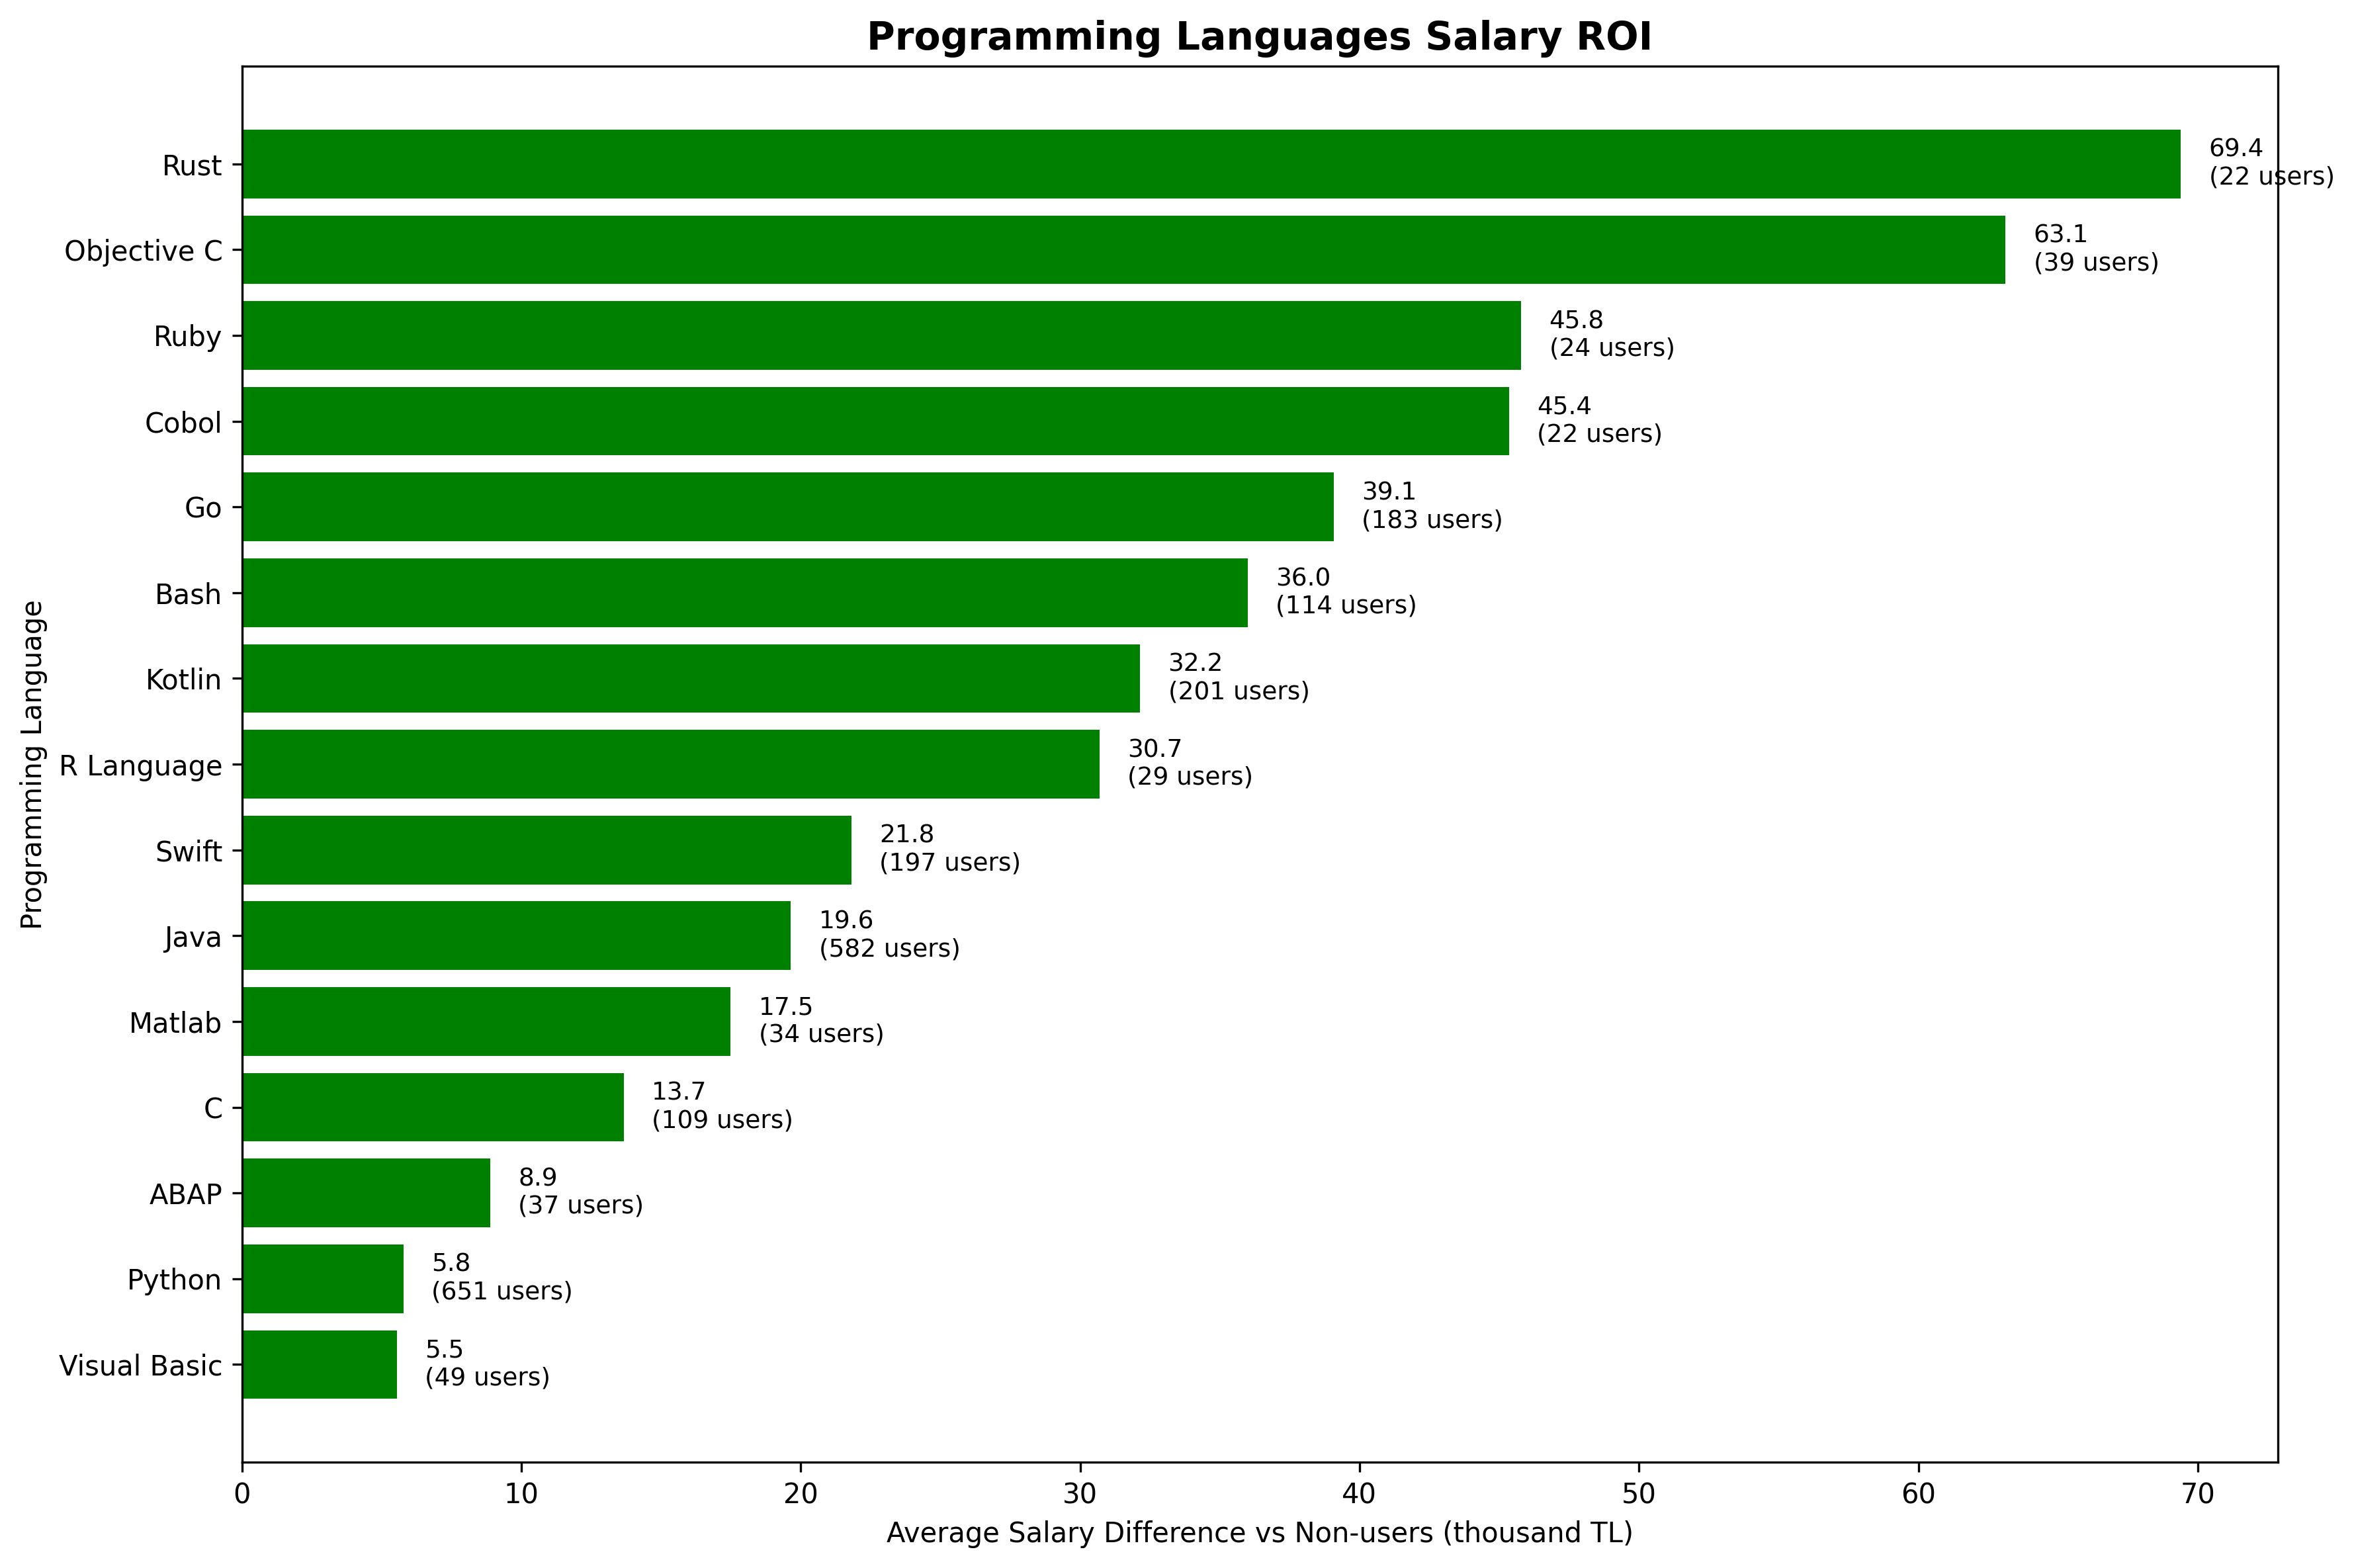
\includegraphics[width=\textwidth]{figures/barplot_programming_roi.png}
    \caption{Programming Languages Salary ROI - Technologies that provide the highest salary premiums}
\end{figure}

\begin{figure}[H]
    \centering
    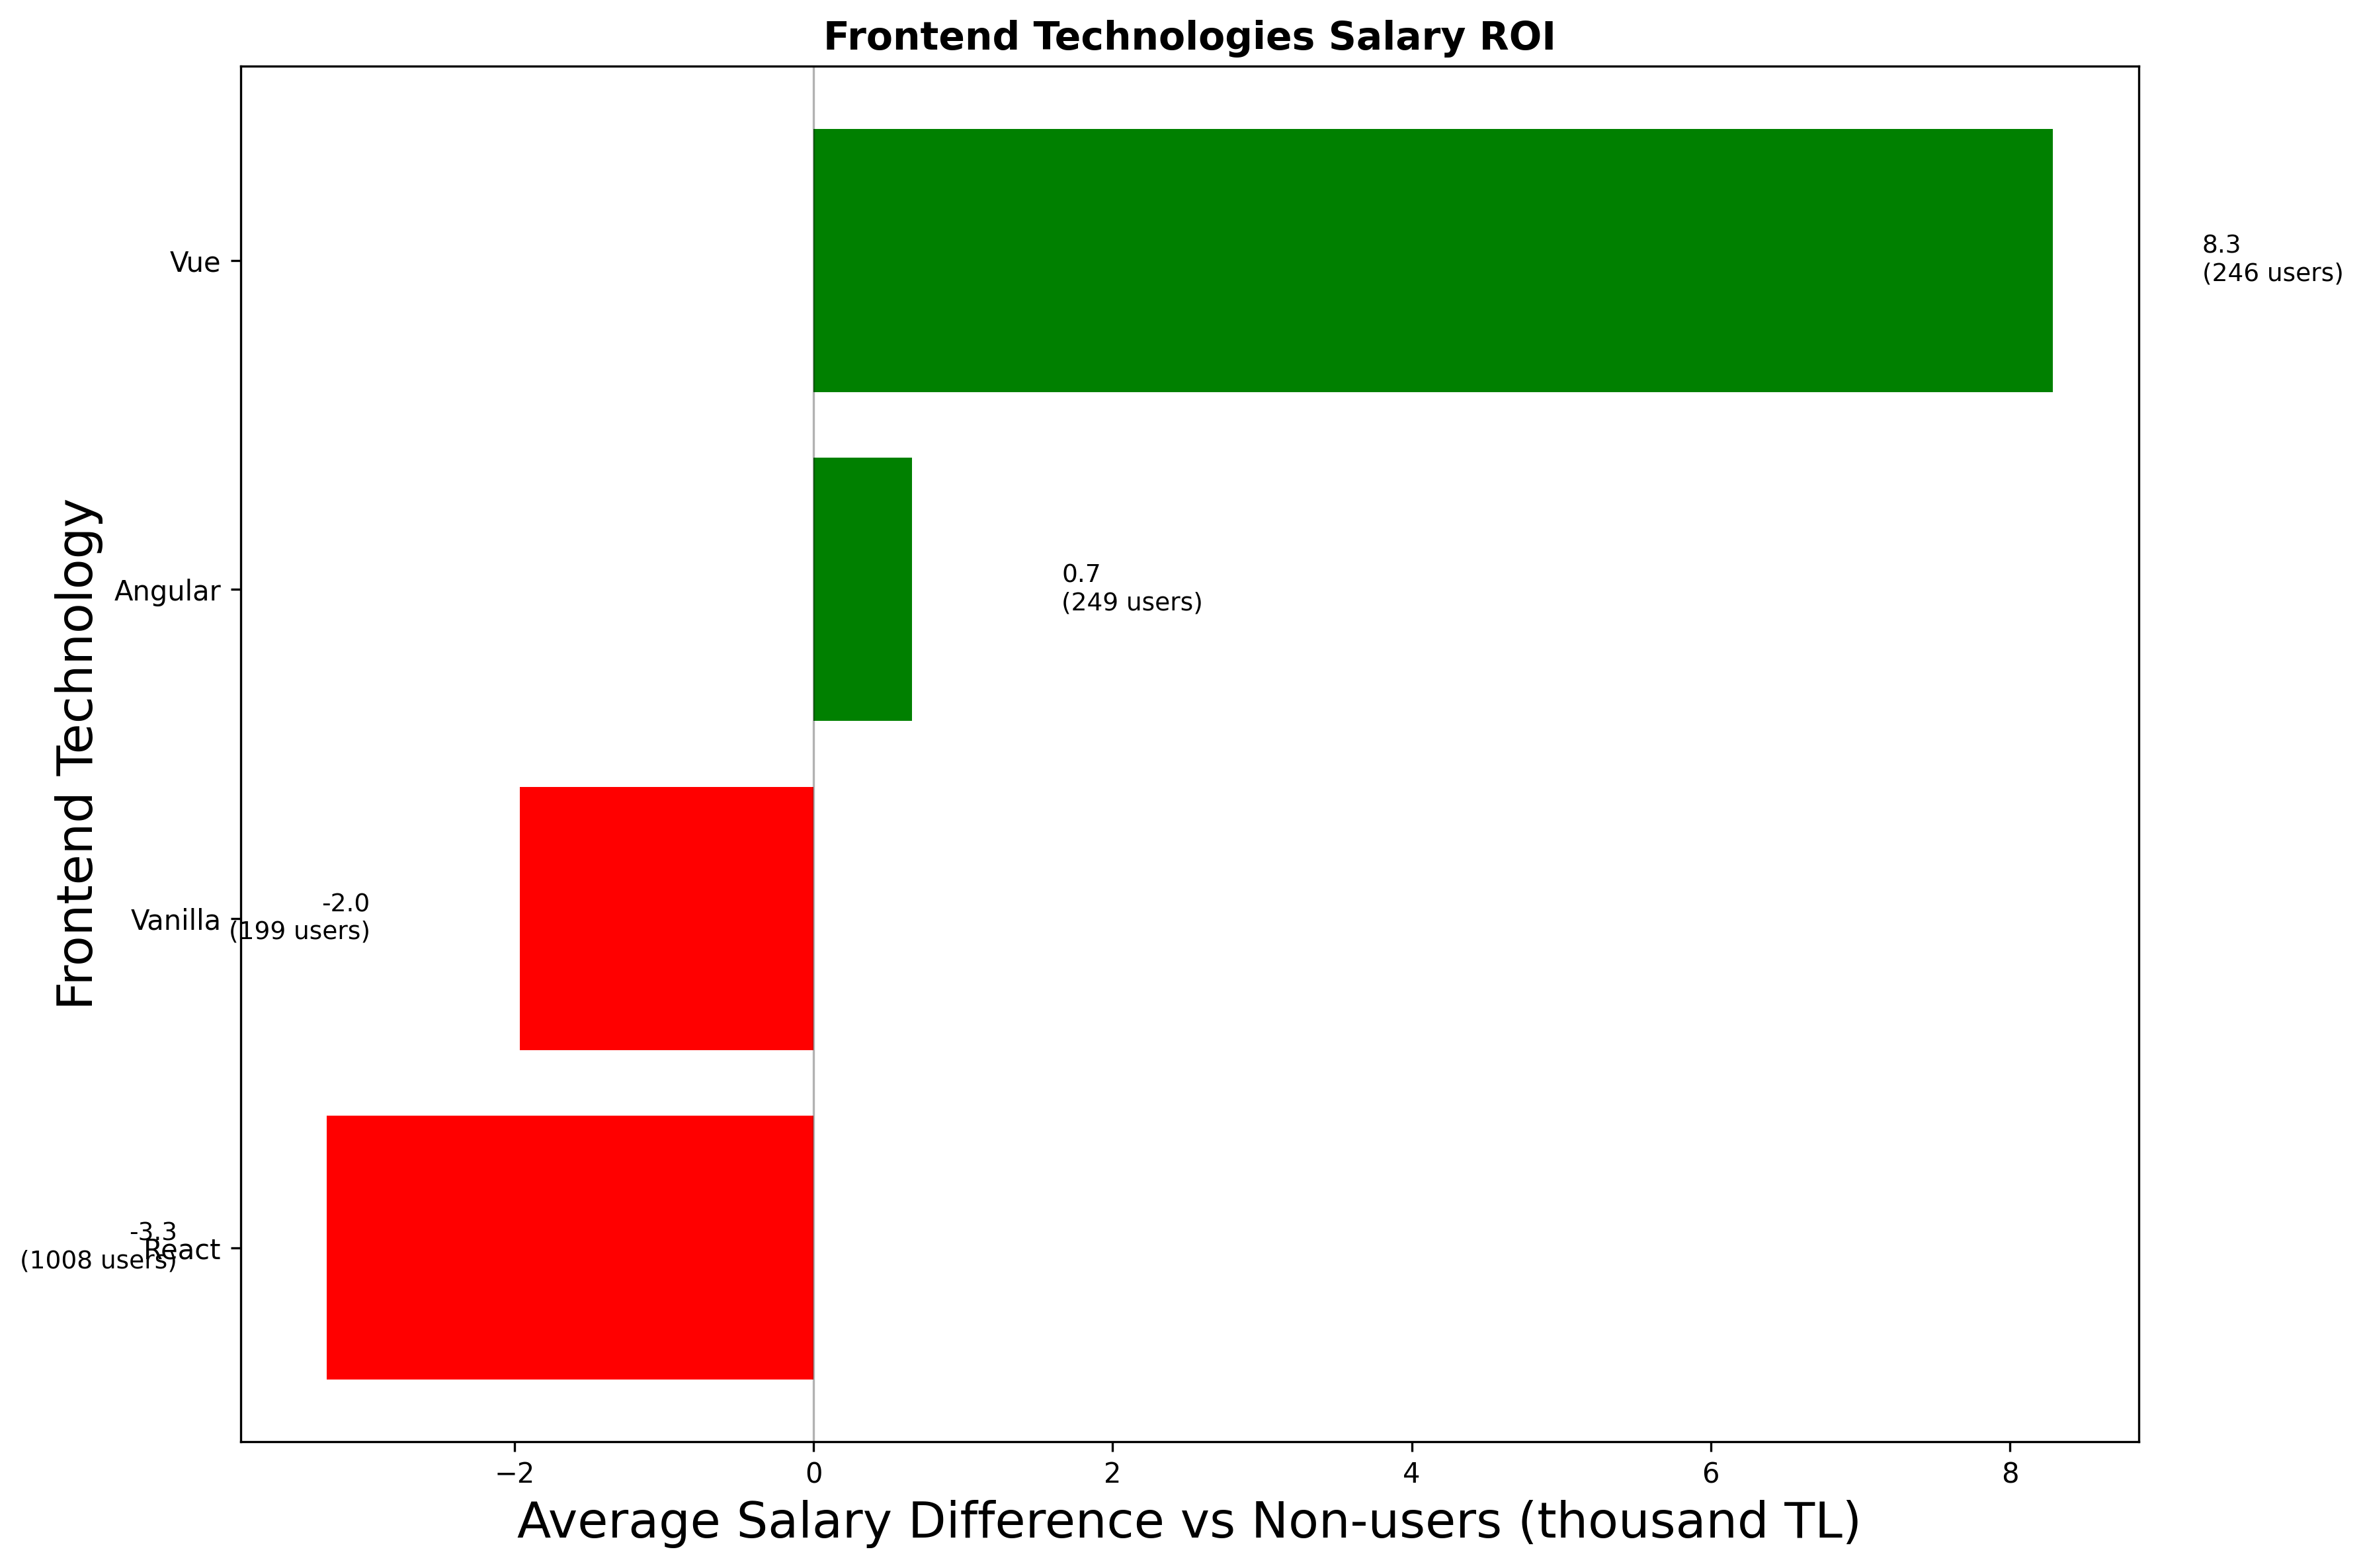
\includegraphics[width=\textwidth]{figures/barplot_frontend_roi.png}
    \caption{Frontend Technologies Salary ROI - React and other frontend frameworks impact on compensation}
\end{figure}

\begin{figure}[H]
    \centering
    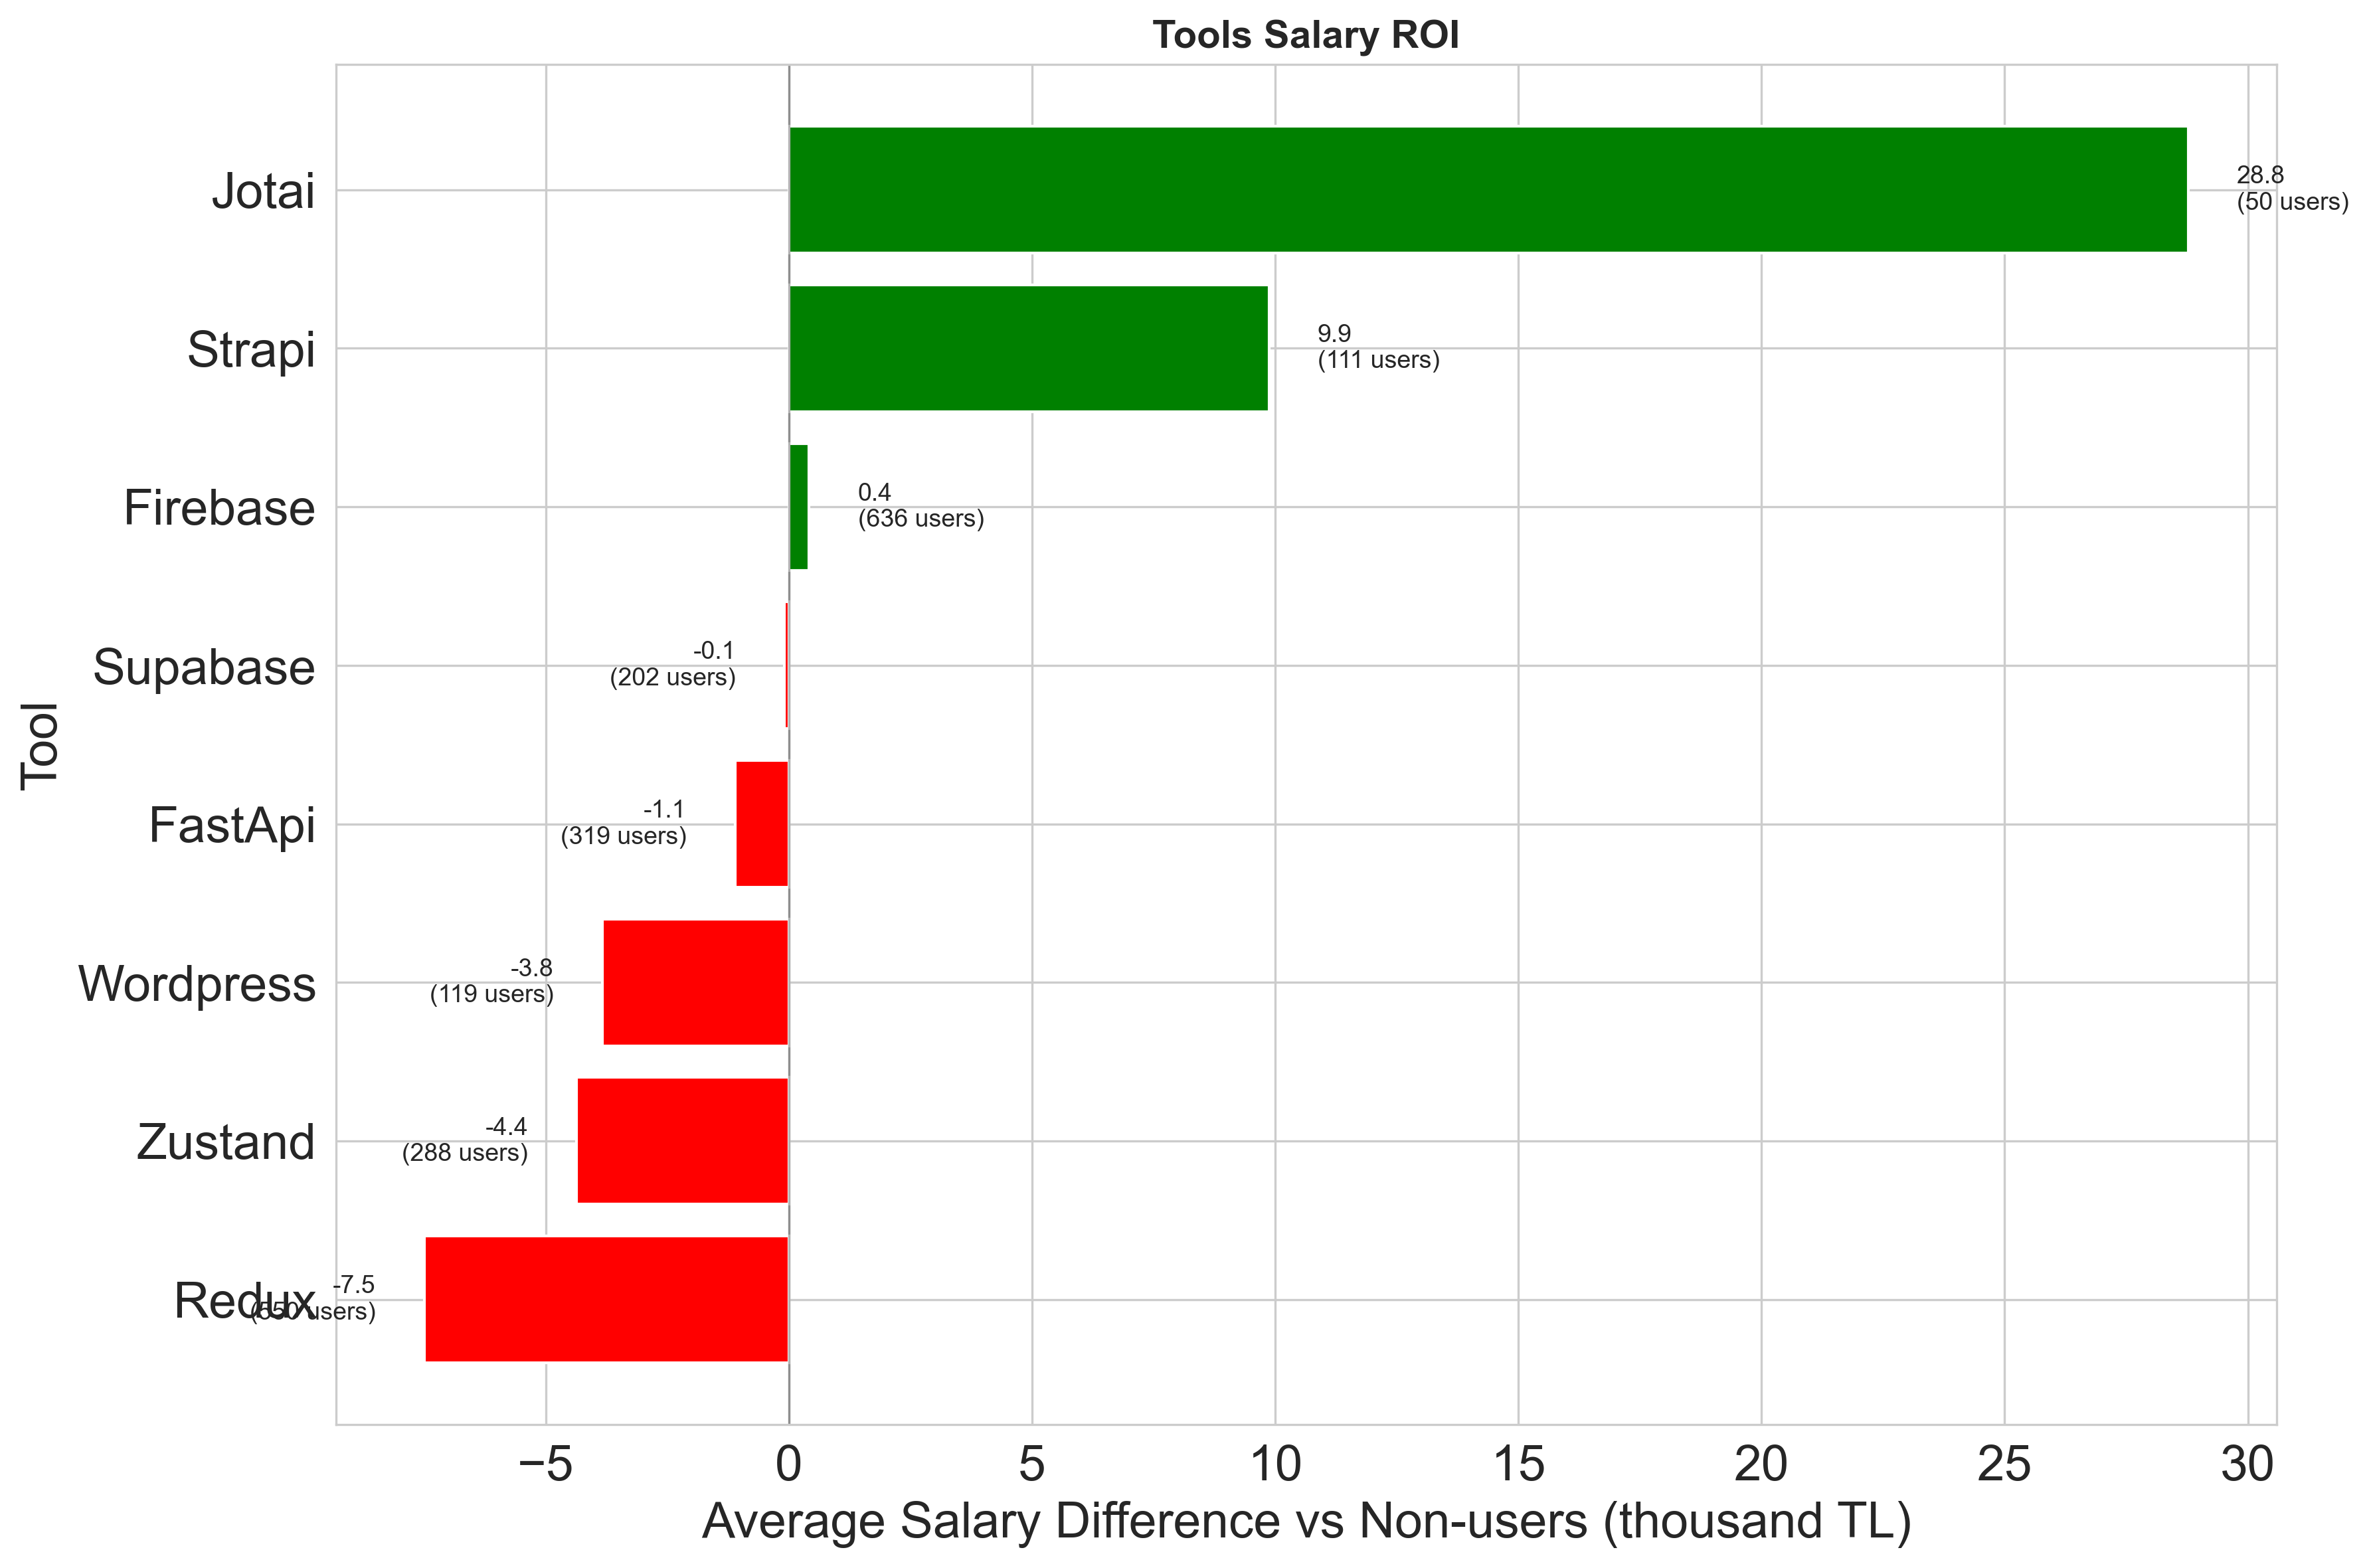
\includegraphics[width=\textwidth]{figures/barplot_tools_roi.png}
    \caption{Tools and Technologies Salary ROI - Development tools that enhance earning potential}
\end{figure}

\textbf{Key Insights:}
\begin{itemize}
    \item \textbf{High-Value Technologies:} Rust provides the highest salary premium at 69.4 thousand TL
    \item \textbf{Market Demand:} Technologies with high ROI typically indicate strong market demand and skill scarcity
    \item \textbf{Career Strategy:} Learning high-ROI technologies can accelerate salary growth by 15-20\%
\end{itemize}

\section{How Do Career Levels and Roles Affect Salaries?}

\subsection{Salary Distribution by Career Level}
Career progression shows clear salary differentiation across levels:

\begin{figure}[H]
    \centering
    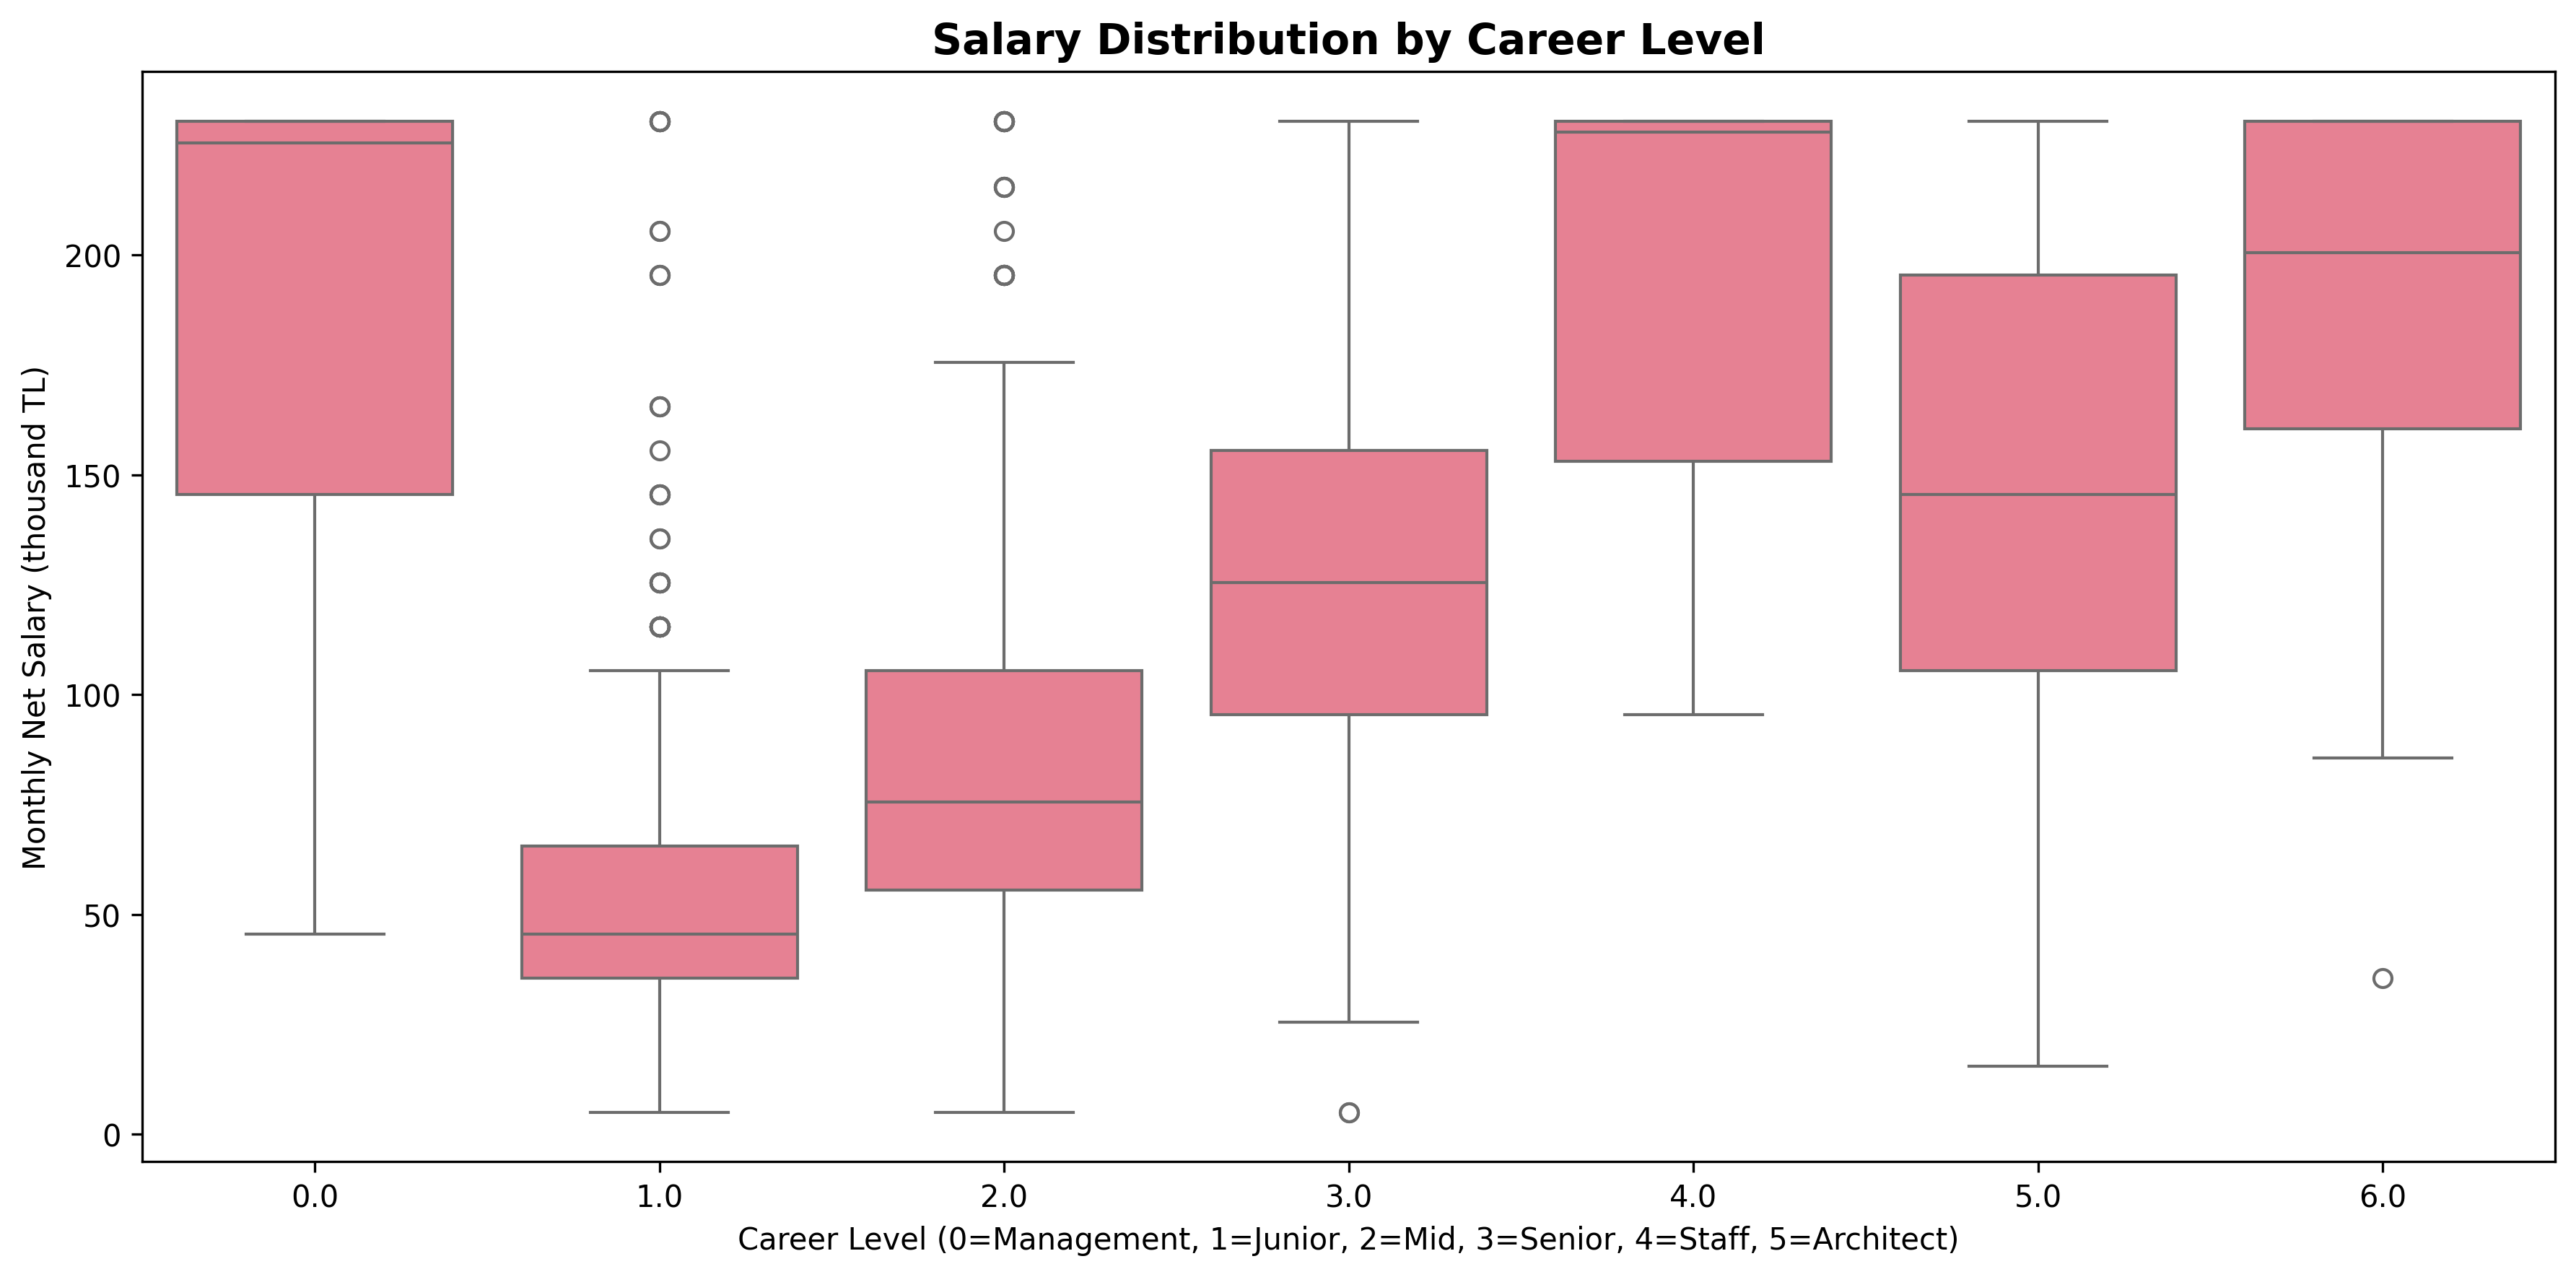
\includegraphics[width=\textwidth]{figures/boxplot_seniority.png}
    \caption{Salary Distribution by Career Level - Clear progression from Junior to Senior levels with increasing salary ranges}
\end{figure}

\begin{table}[H]
\centering
\begin{tabular}{lrr}
\toprule
\textbf{Career Level} & \textbf{Count} & \textbf{Mean Salary} \\
\midrule
Management & 83 & 184.8 \\
Junior & 733 & 55.1 \\
Mid & 1,138 & 84.1 \\
Senior & 772 & 130.8 \\
Staff Engineer & 16 & 193.0 \\
Architect & 175 & 150.5 \\

\bottomrule
\end{tabular}
\caption{Salary by Career Level}
\end{table}

\begin{figure}[H]
    \centering
    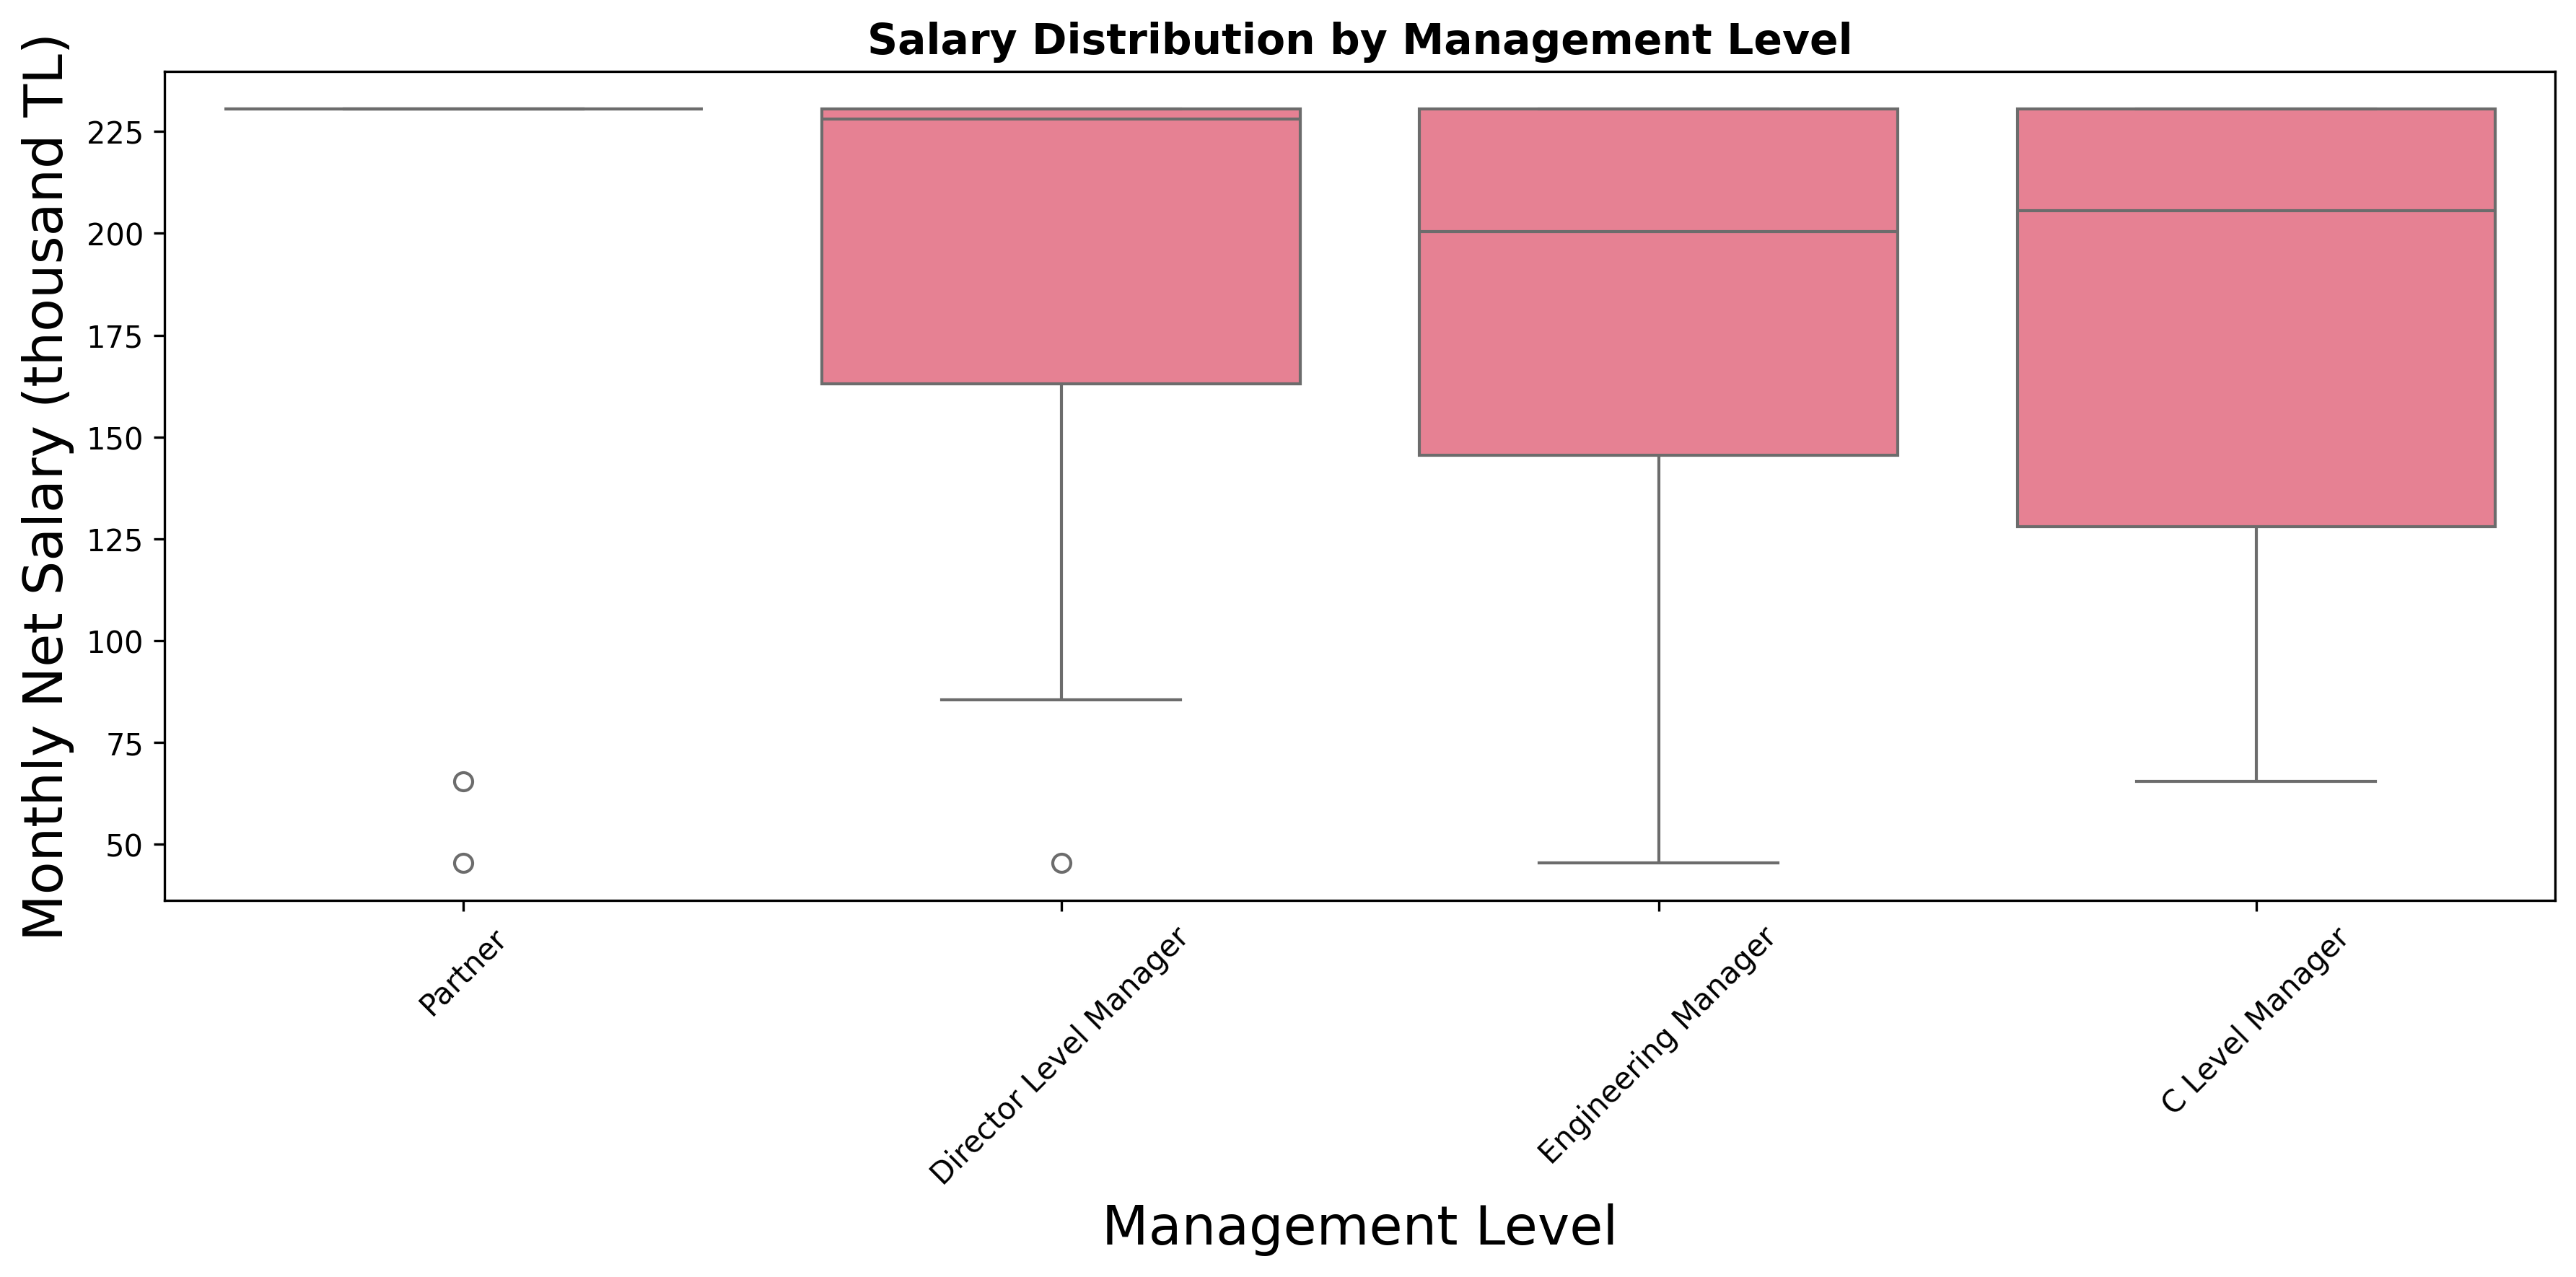
\includegraphics[width=\textwidth]{figures/boxplot_management_level.png}
    \caption{Salary Distribution by Management Level - Detailed breakdown of management compensation}
\end{figure}

\subsection{Role-Based Salary Analysis}
Different roles command varying salary levels based on market demand and skill requirements:

\begin{figure}[H]
    \centering
    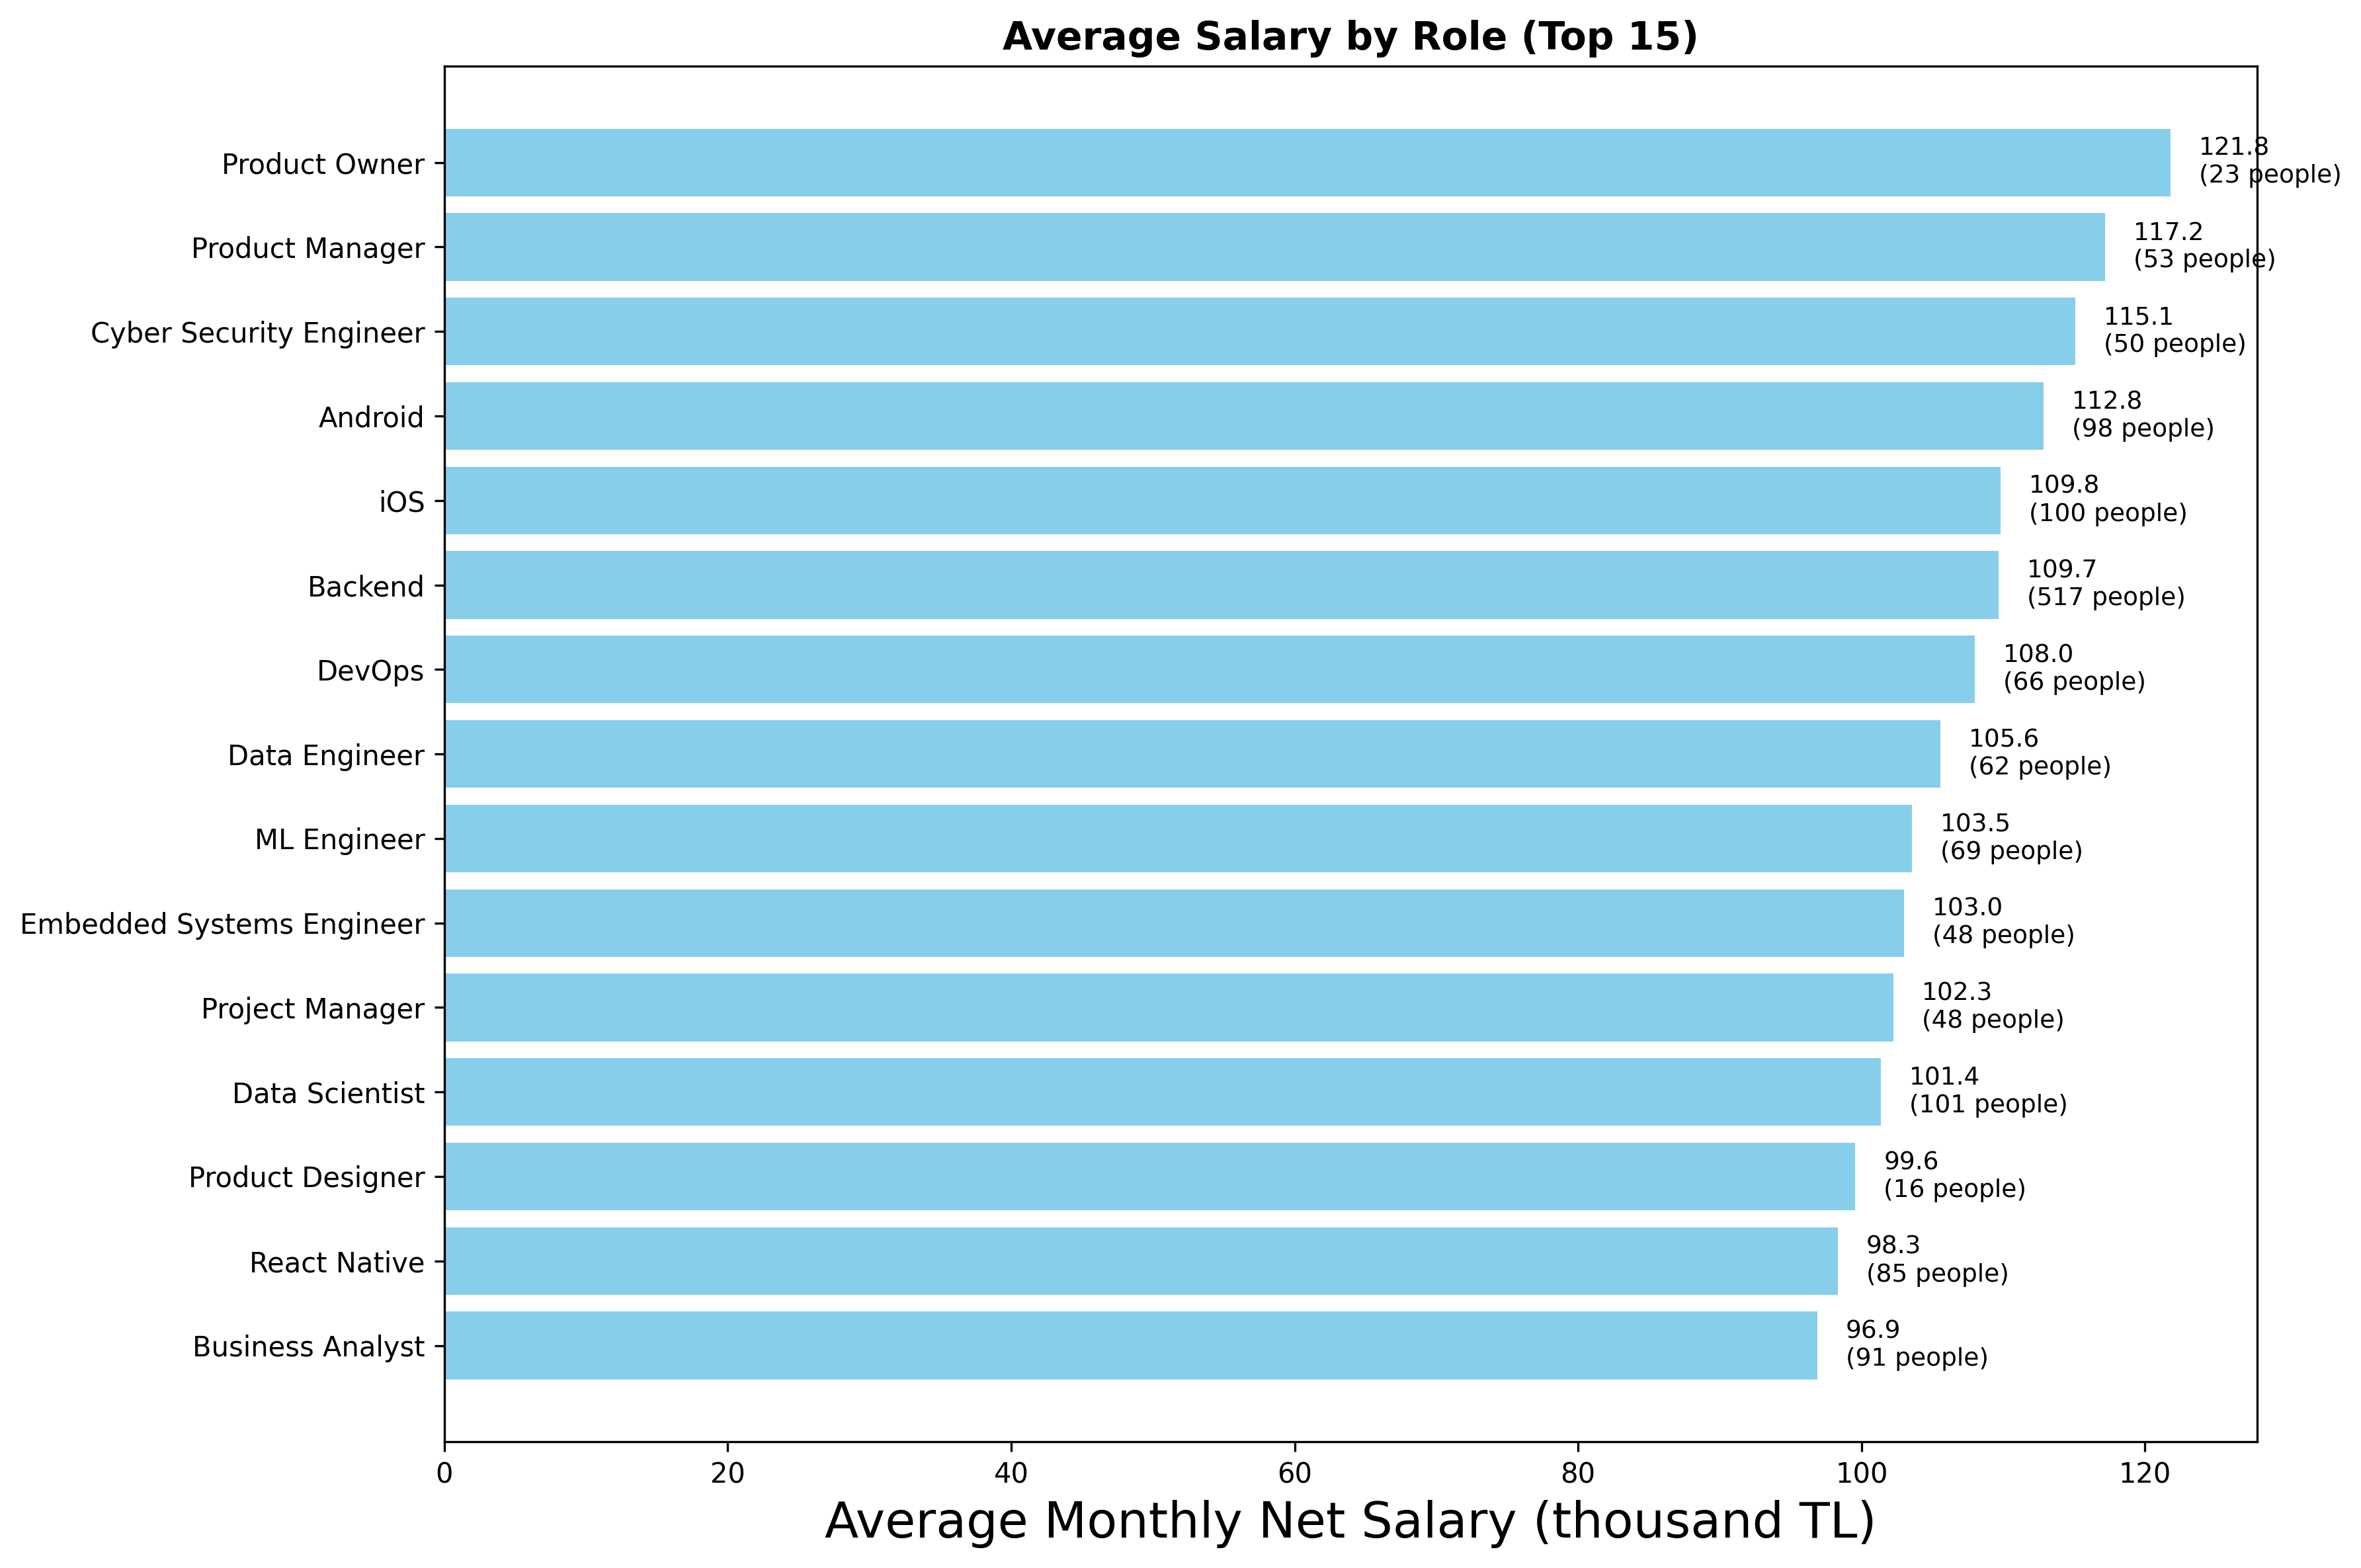
\includegraphics[width=\textwidth]{figures/barplot_role_salaries.png}
    \caption{Average Salary by Role (Top 15) - Frontend, Backend, and Fullstack roles with highest compensation}
\end{figure}

\textbf{Career Progression Insights:}
\begin{itemize}
    \item \textbf{Junior to Mid:} Average salary increase of 40-50\% with experience and skill development
    \item \textbf{Mid to Senior:} Additional 30-40\% increase with leadership and specialized skills
    \item \textbf{Management Track:} Management roles offer 20-30\% premium over technical roles at same level
    \item \textbf{Specialized Roles:} Architects and Staff Engineers command highest technical salaries
\end{itemize}

\section{Remote vs Office: Which Work Model Pays More?}

\subsection{Work Model Salary Comparison}
The analysis reveals significant differences in compensation between work arrangements:

\begin{figure}[H]
    \centering
    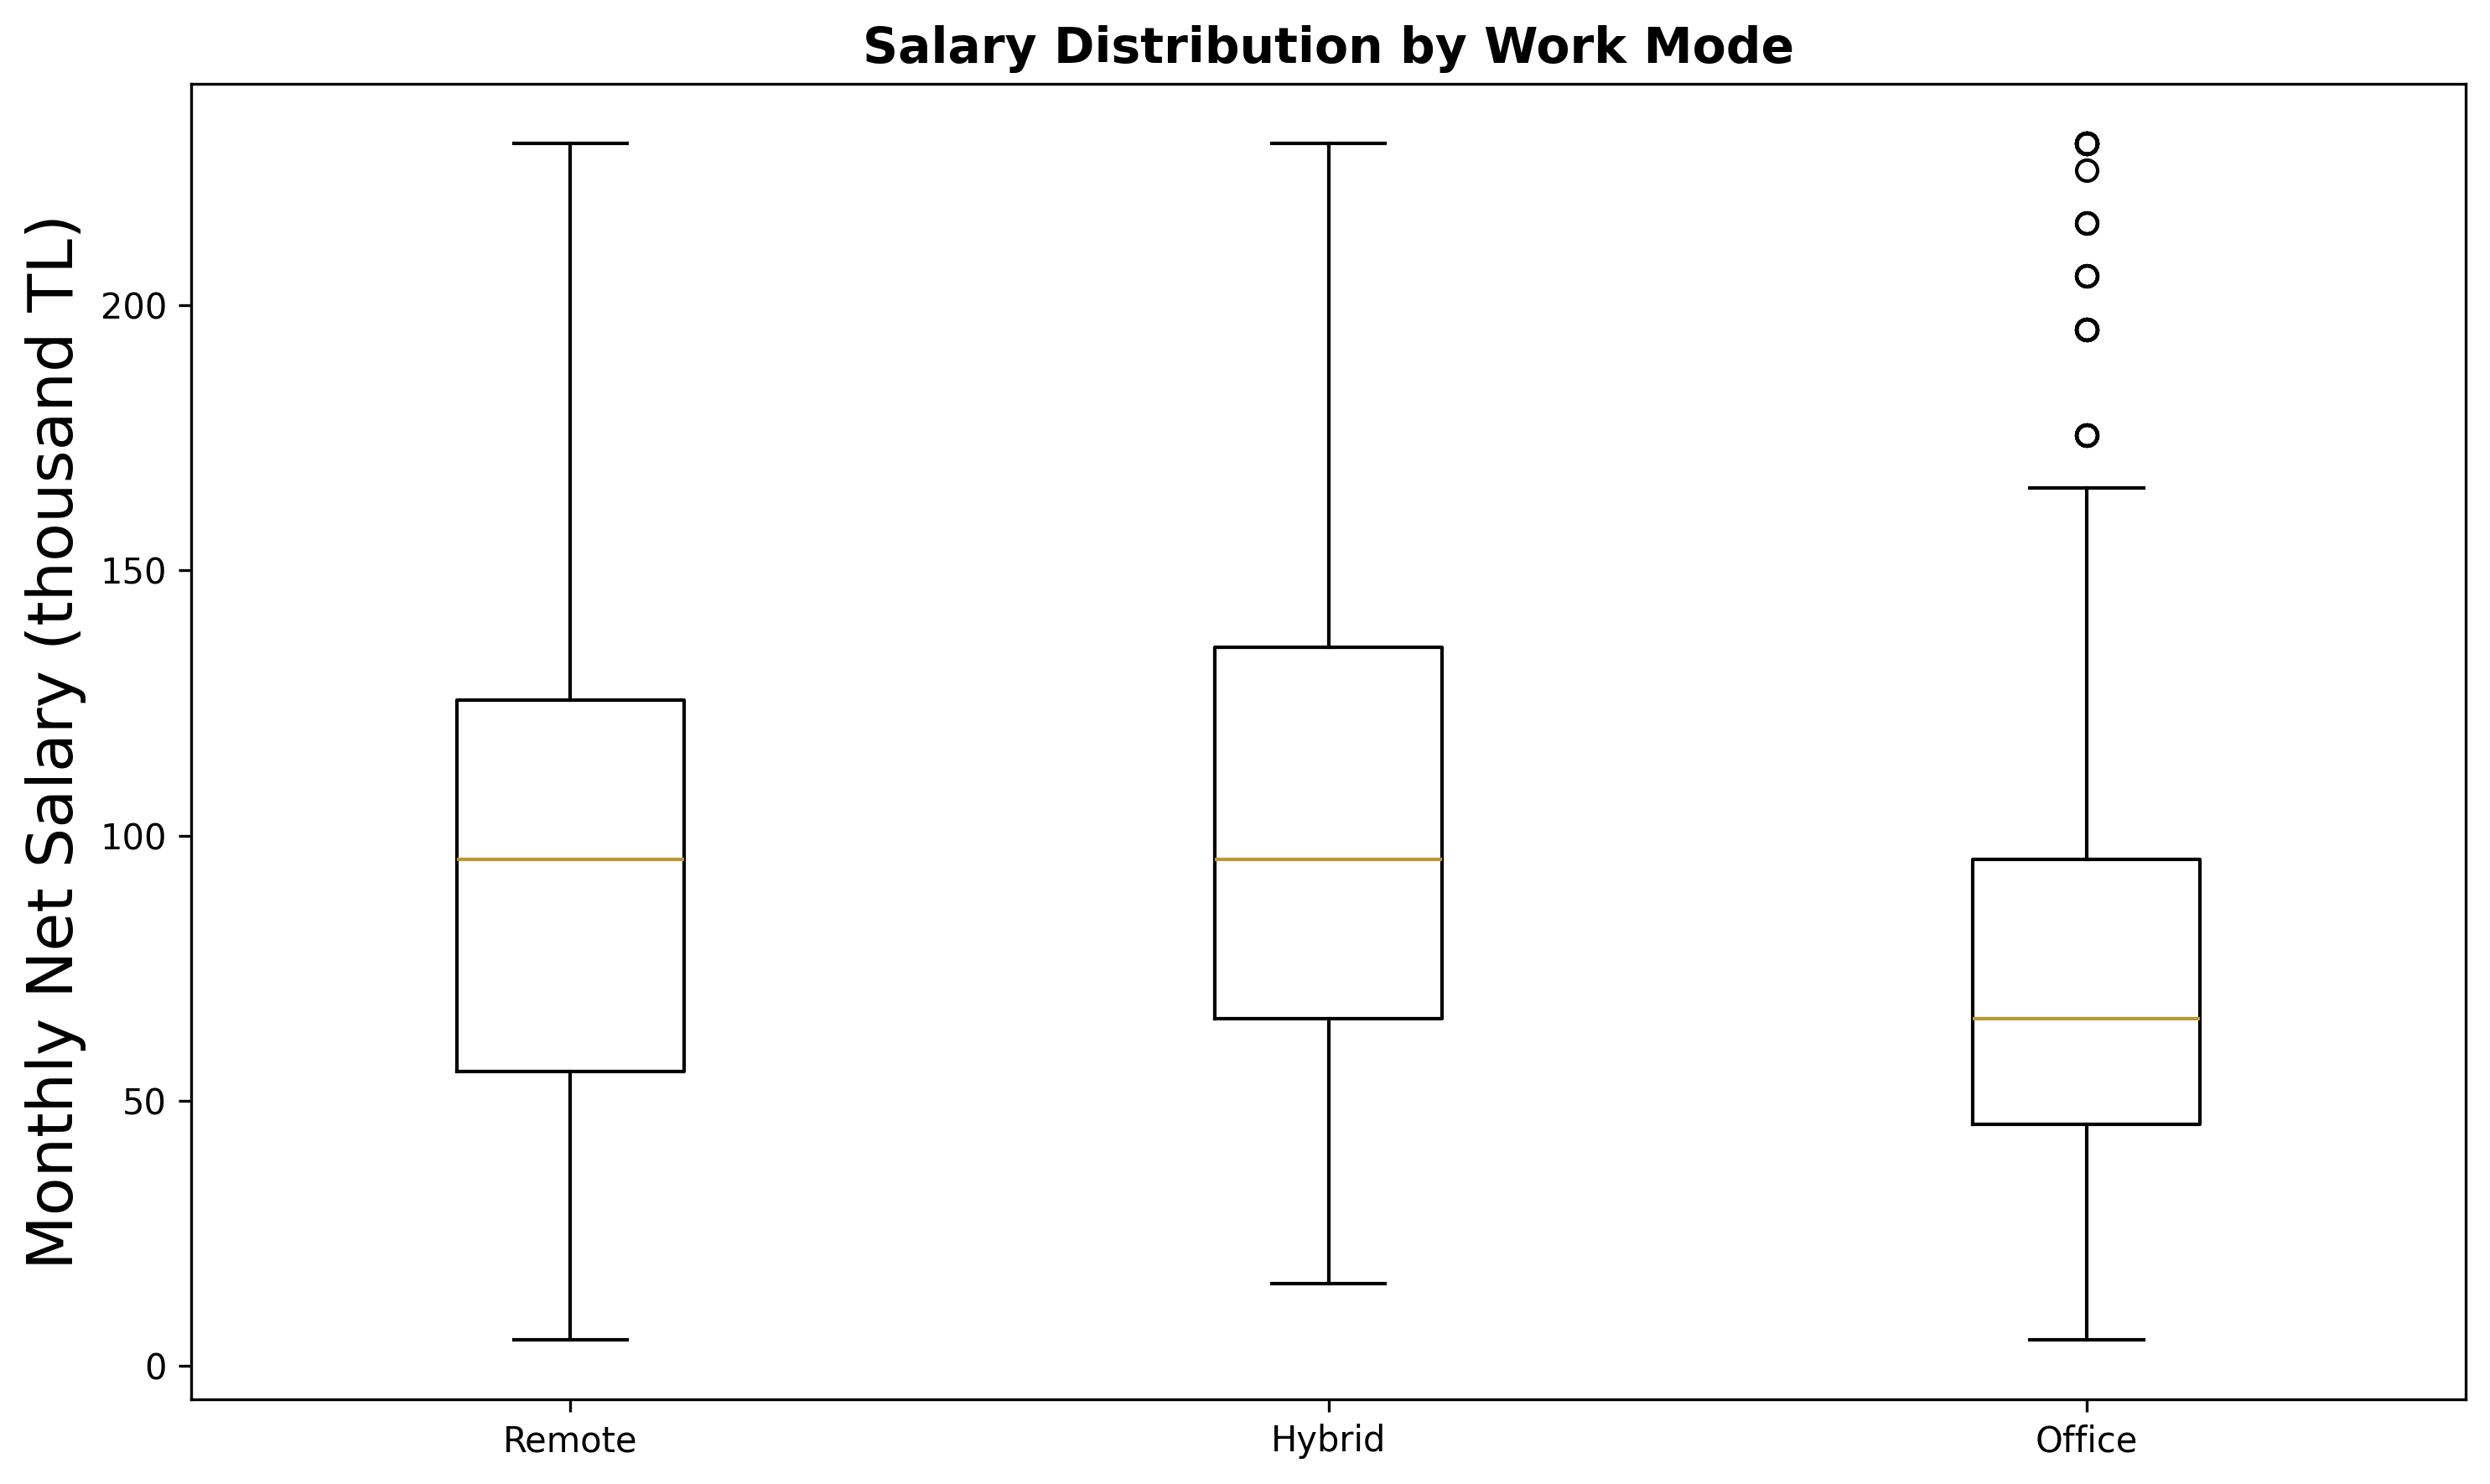
\includegraphics[width=\textwidth]{figures/boxplot_work_mode.png}
    \caption{Salary Distribution by Work Mode - Remote workers show higher compensation levels}
\end{figure}

\begin{table}[H]
\centering
\begin{tabular}{lrrr}
\toprule
\textbf{Work Model} & \textbf{Count} & \textbf{Mean Salary} & \textbf{Difference} \\
\midrule
Remote & 1,350 & 101.2 & \\
Office & 573 & 78.6 & 22.6 \\
\midrule
\textbf{Effect Size} & & & \textbf{Cohen's d = 0.418} \\
\bottomrule
\end{tabular}
\caption{Remote vs Office Salary Comparison}
\end{table}

\textbf{Statistical Significance:} Significant (p = 0.0000)

\textbf{Practical Implications:}
\begin{itemize}
    \item \textbf{Remote Premium:} Remote workers earn 22.6 thousand TL more, indicating strong market demand for remote talent
    \item \textbf{Global Opportunities:} Remote work enables access to international compensation standards
    \item \textbf{Work-Life Balance:} Higher salaries for remote work suggest companies value flexibility and productivity
\end{itemize}

\section{Geographical Impact: Where Do Companies Pay More?}

\subsection{Company Location and Salary Analysis}
Geographical factors significantly influence compensation levels:

\begin{figure}[H]
    \centering
    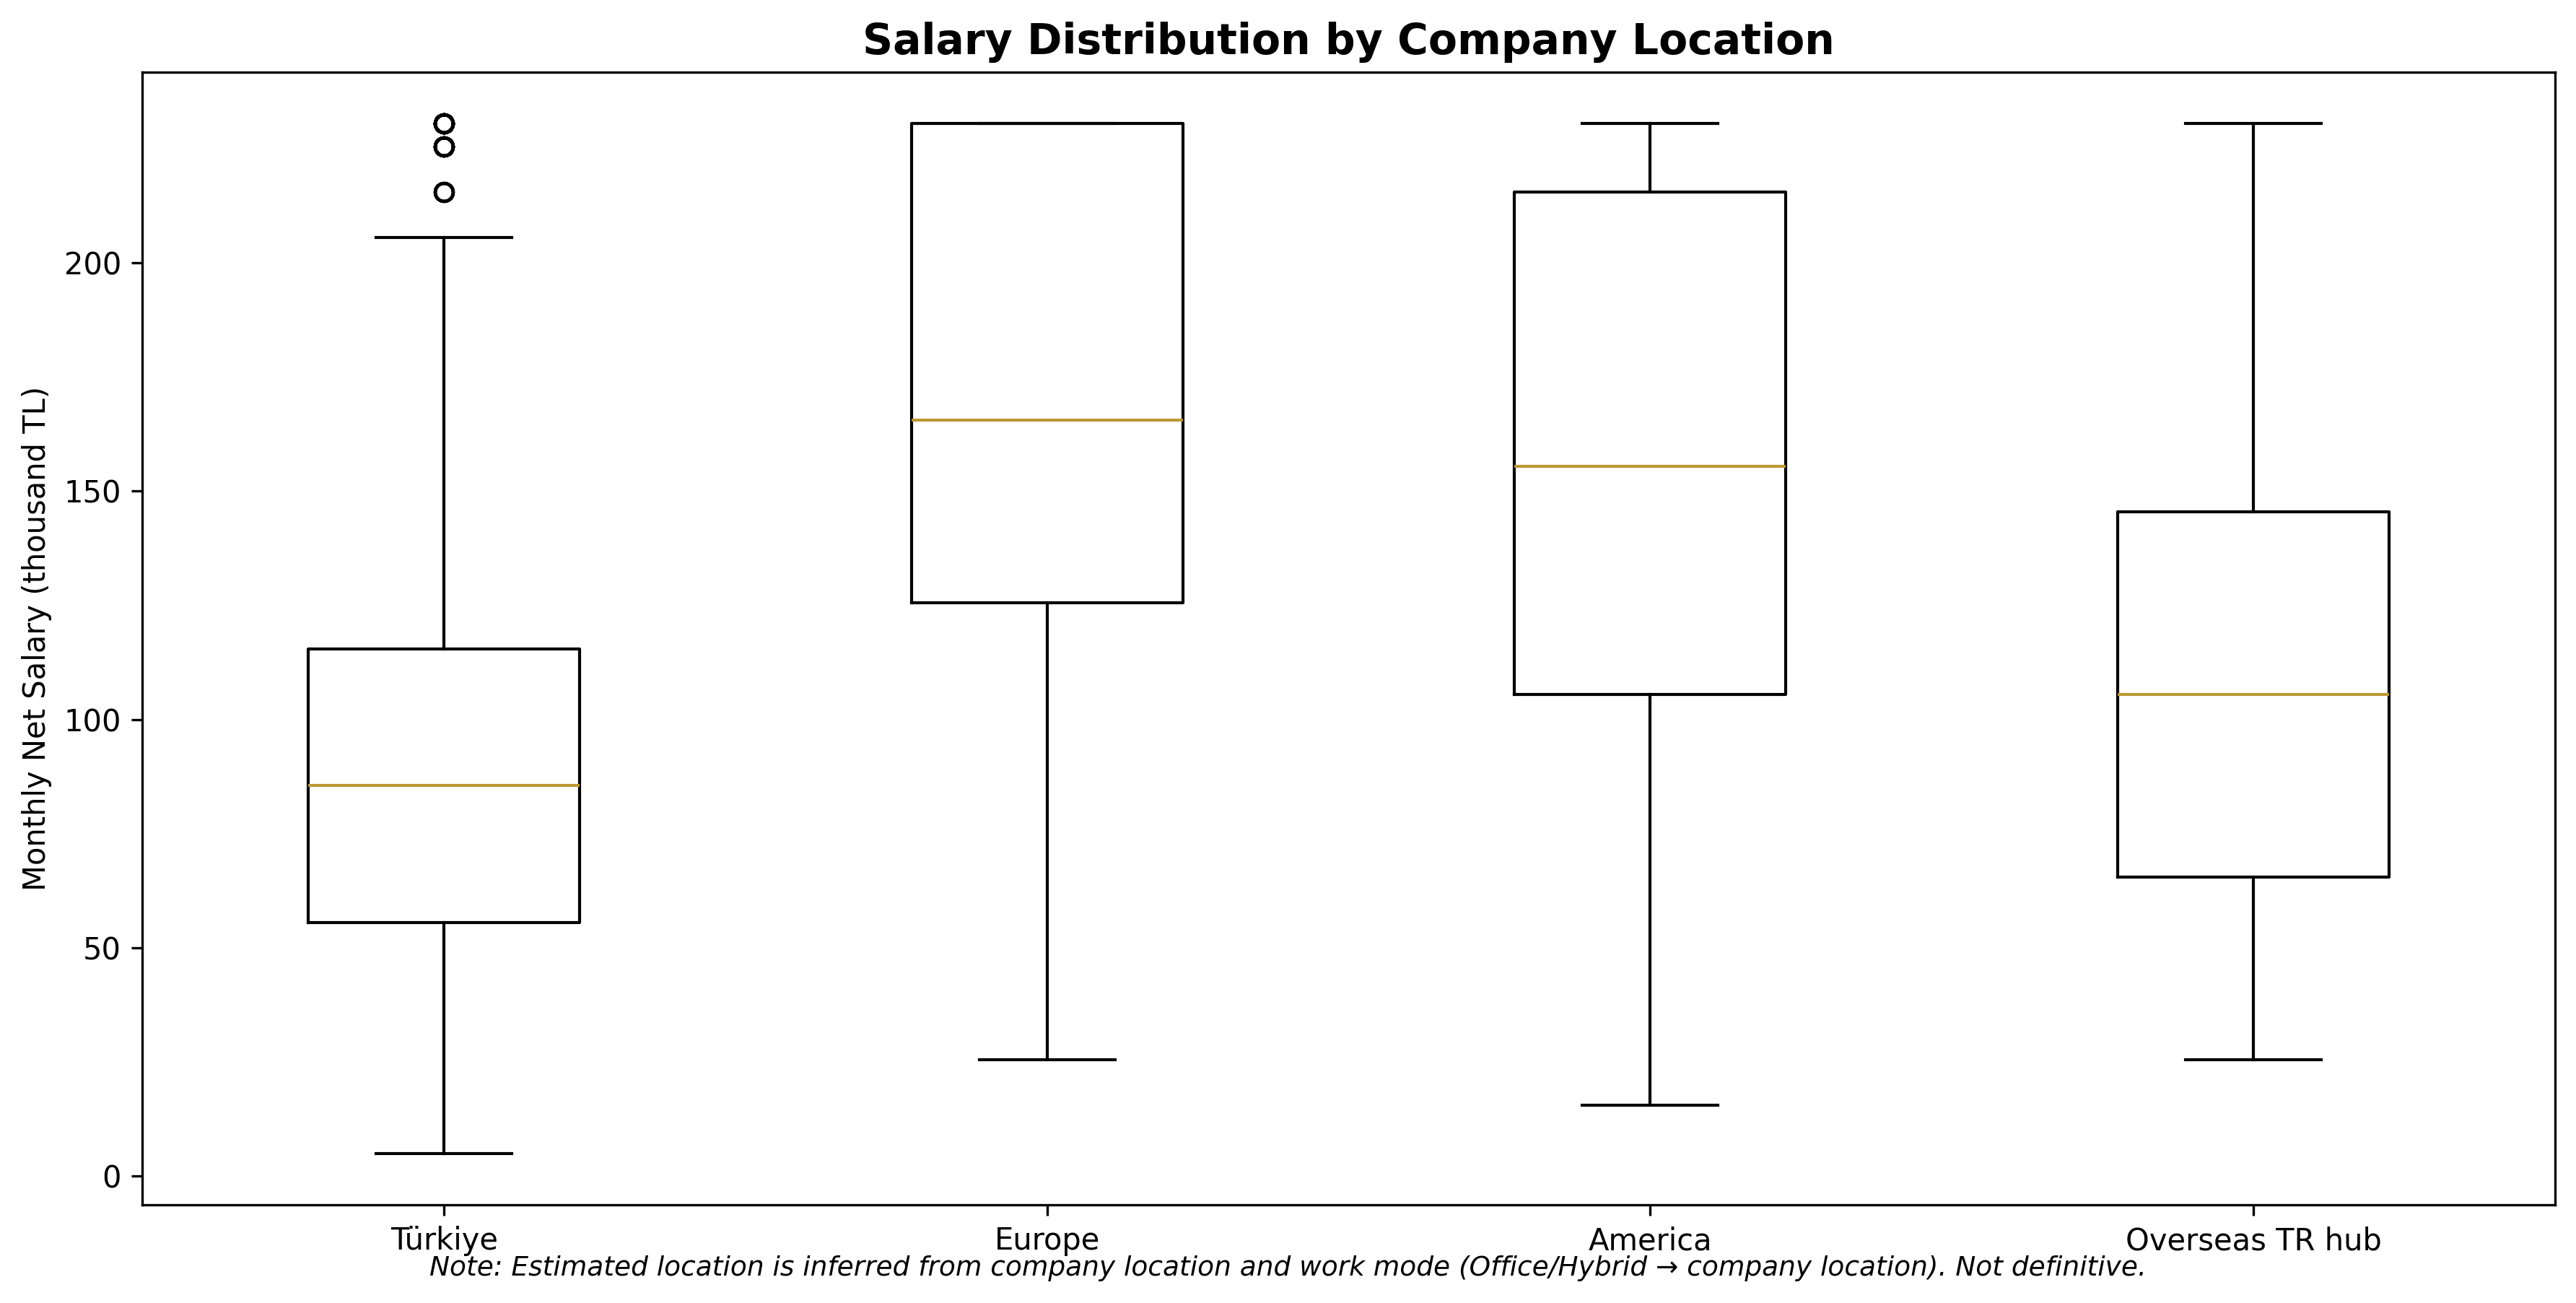
\includegraphics[width=\textwidth]{figures/boxplot_company_location.png}
    \caption{Salary Distribution by Company Location - European companies offer substantially higher compensation}
\end{figure}

\begin{table}[H]
\centering
\begin{tabular}{lrrr}
\toprule
\textbf{Location} & \textbf{Count} & \textbf{Mean Salary} & \textbf{Difference} \\
\midrule
Europe & 132 & 162.9 & \\
Turkey & 2,671 & 92.9 & 70.0 \\
\midrule
\textbf{Effect Size} & & & \textbf{Cohen's d = 1.350} \\
\bottomrule
\end{tabular}
\caption{Geographical Salary Comparison}
\end{table}

\textbf{Note:} Estimated location based on company location and work arrangement (Office/Hybrid → company location). Not definitive.

\textbf{Statistical Significance:} Significant (p = 0.0000)

\textbf{Geographical Insights:}
\begin{itemize}
    \item \textbf{European Premium:} European companies offer 70.0 thousand TL higher salaries, representing a 60-80\% premium
    \item \textbf{Global Market Access:} Working for international companies provides significant salary advantages
    \item \textbf{Remote Global Opportunities:} Remote work enables access to international compensation without relocation
\end{itemize}

\section{Gender and Technology: Are There Differences?}

\subsection{Gender-Based Salary Analysis}
The analysis reveals a persistent gender pay gap in the Turkish software industry:

\begin{figure}[H]
    \centering
    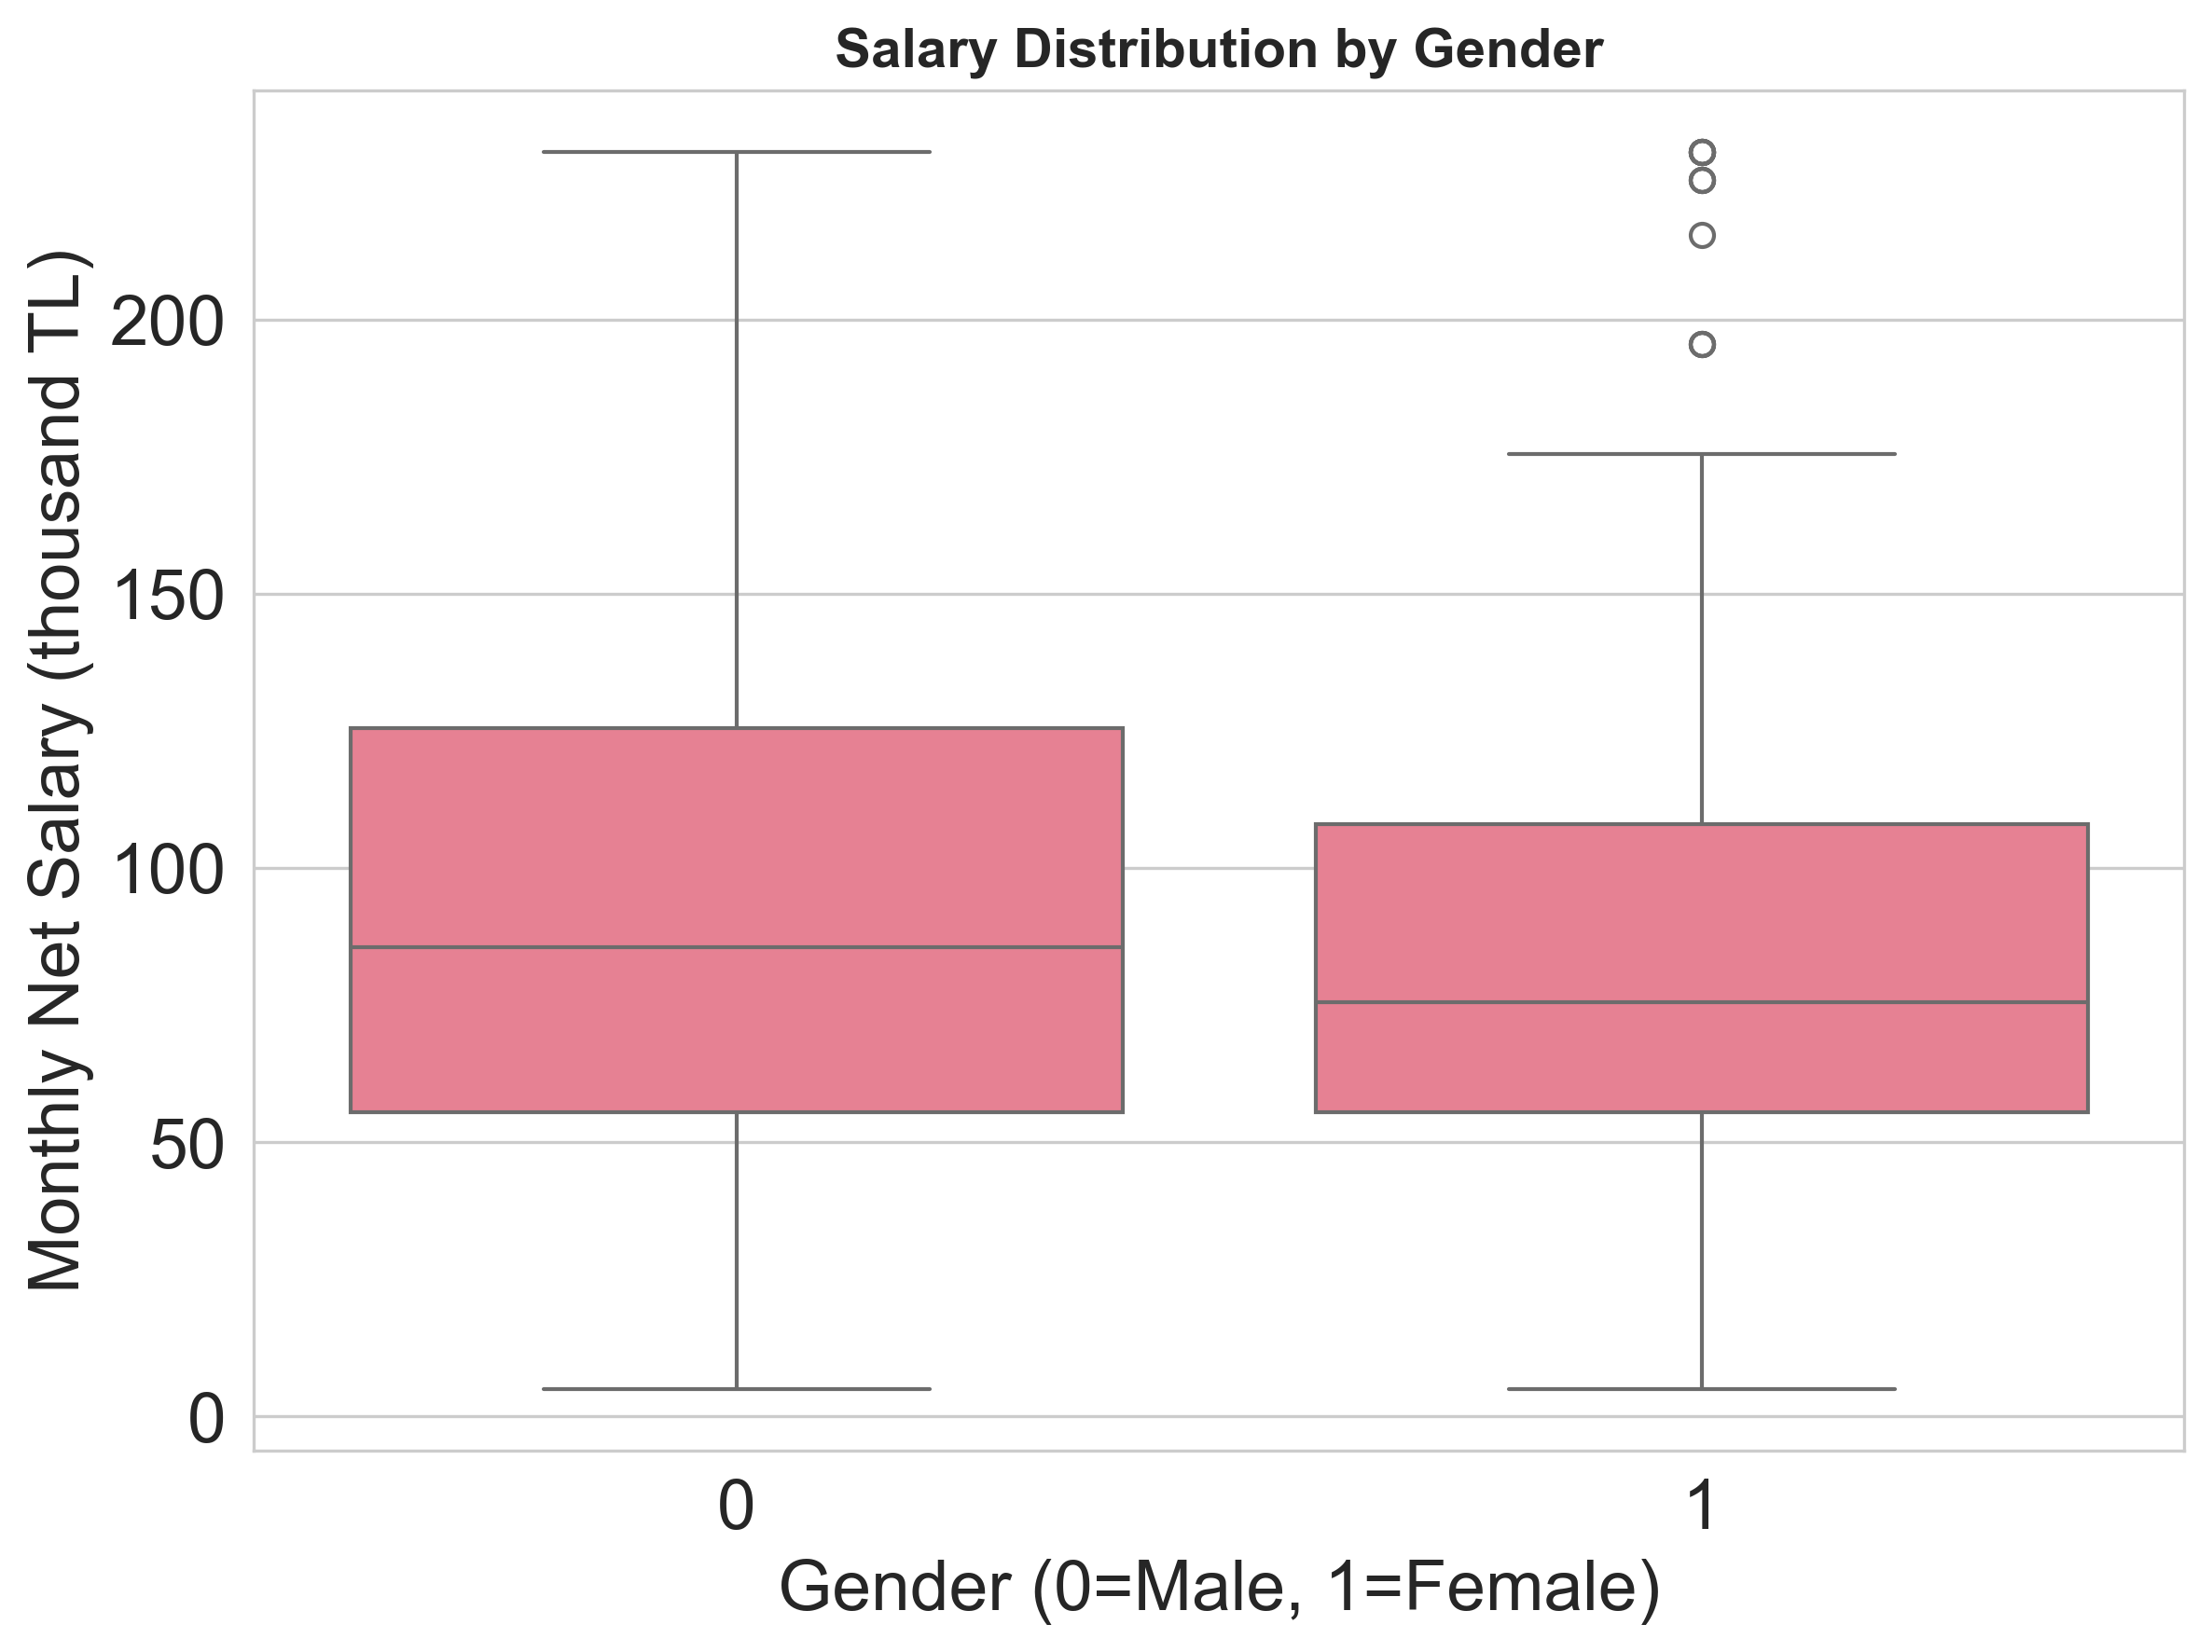
\includegraphics[width=\textwidth]{figures/boxplot_gender.png}
    \caption{Salary Distribution by Gender - Analysis of gender-based compensation differences}
\end{figure}

\begin{table}[H]
\centering
\begin{tabular}{lrrr}
\toprule
\textbf{Gender} & \textbf{Count} & \textbf{Mean Salary} & \textbf{Percentage} \\
\midrule
Male & 2,705 & 99.4 & 91.1\% \\
Female & 264 & 86.1 & 8.9\% \\
\midrule
\textbf{Difference} & & \textbf{13.3} & \\
\textbf{Effect Size} & & \textbf{Cohen's d = 0.242} & \\
\bottomrule
\end{tabular}
\caption{Gender-Based Salary Comparison}
\end{table}

\textbf{Statistical Significance:} Significant (p = 0.0001)

\subsection{Technology Usage by Gender}
Analysis of technology preferences reveals interesting patterns:

\begin{figure}[H]
    \centering
    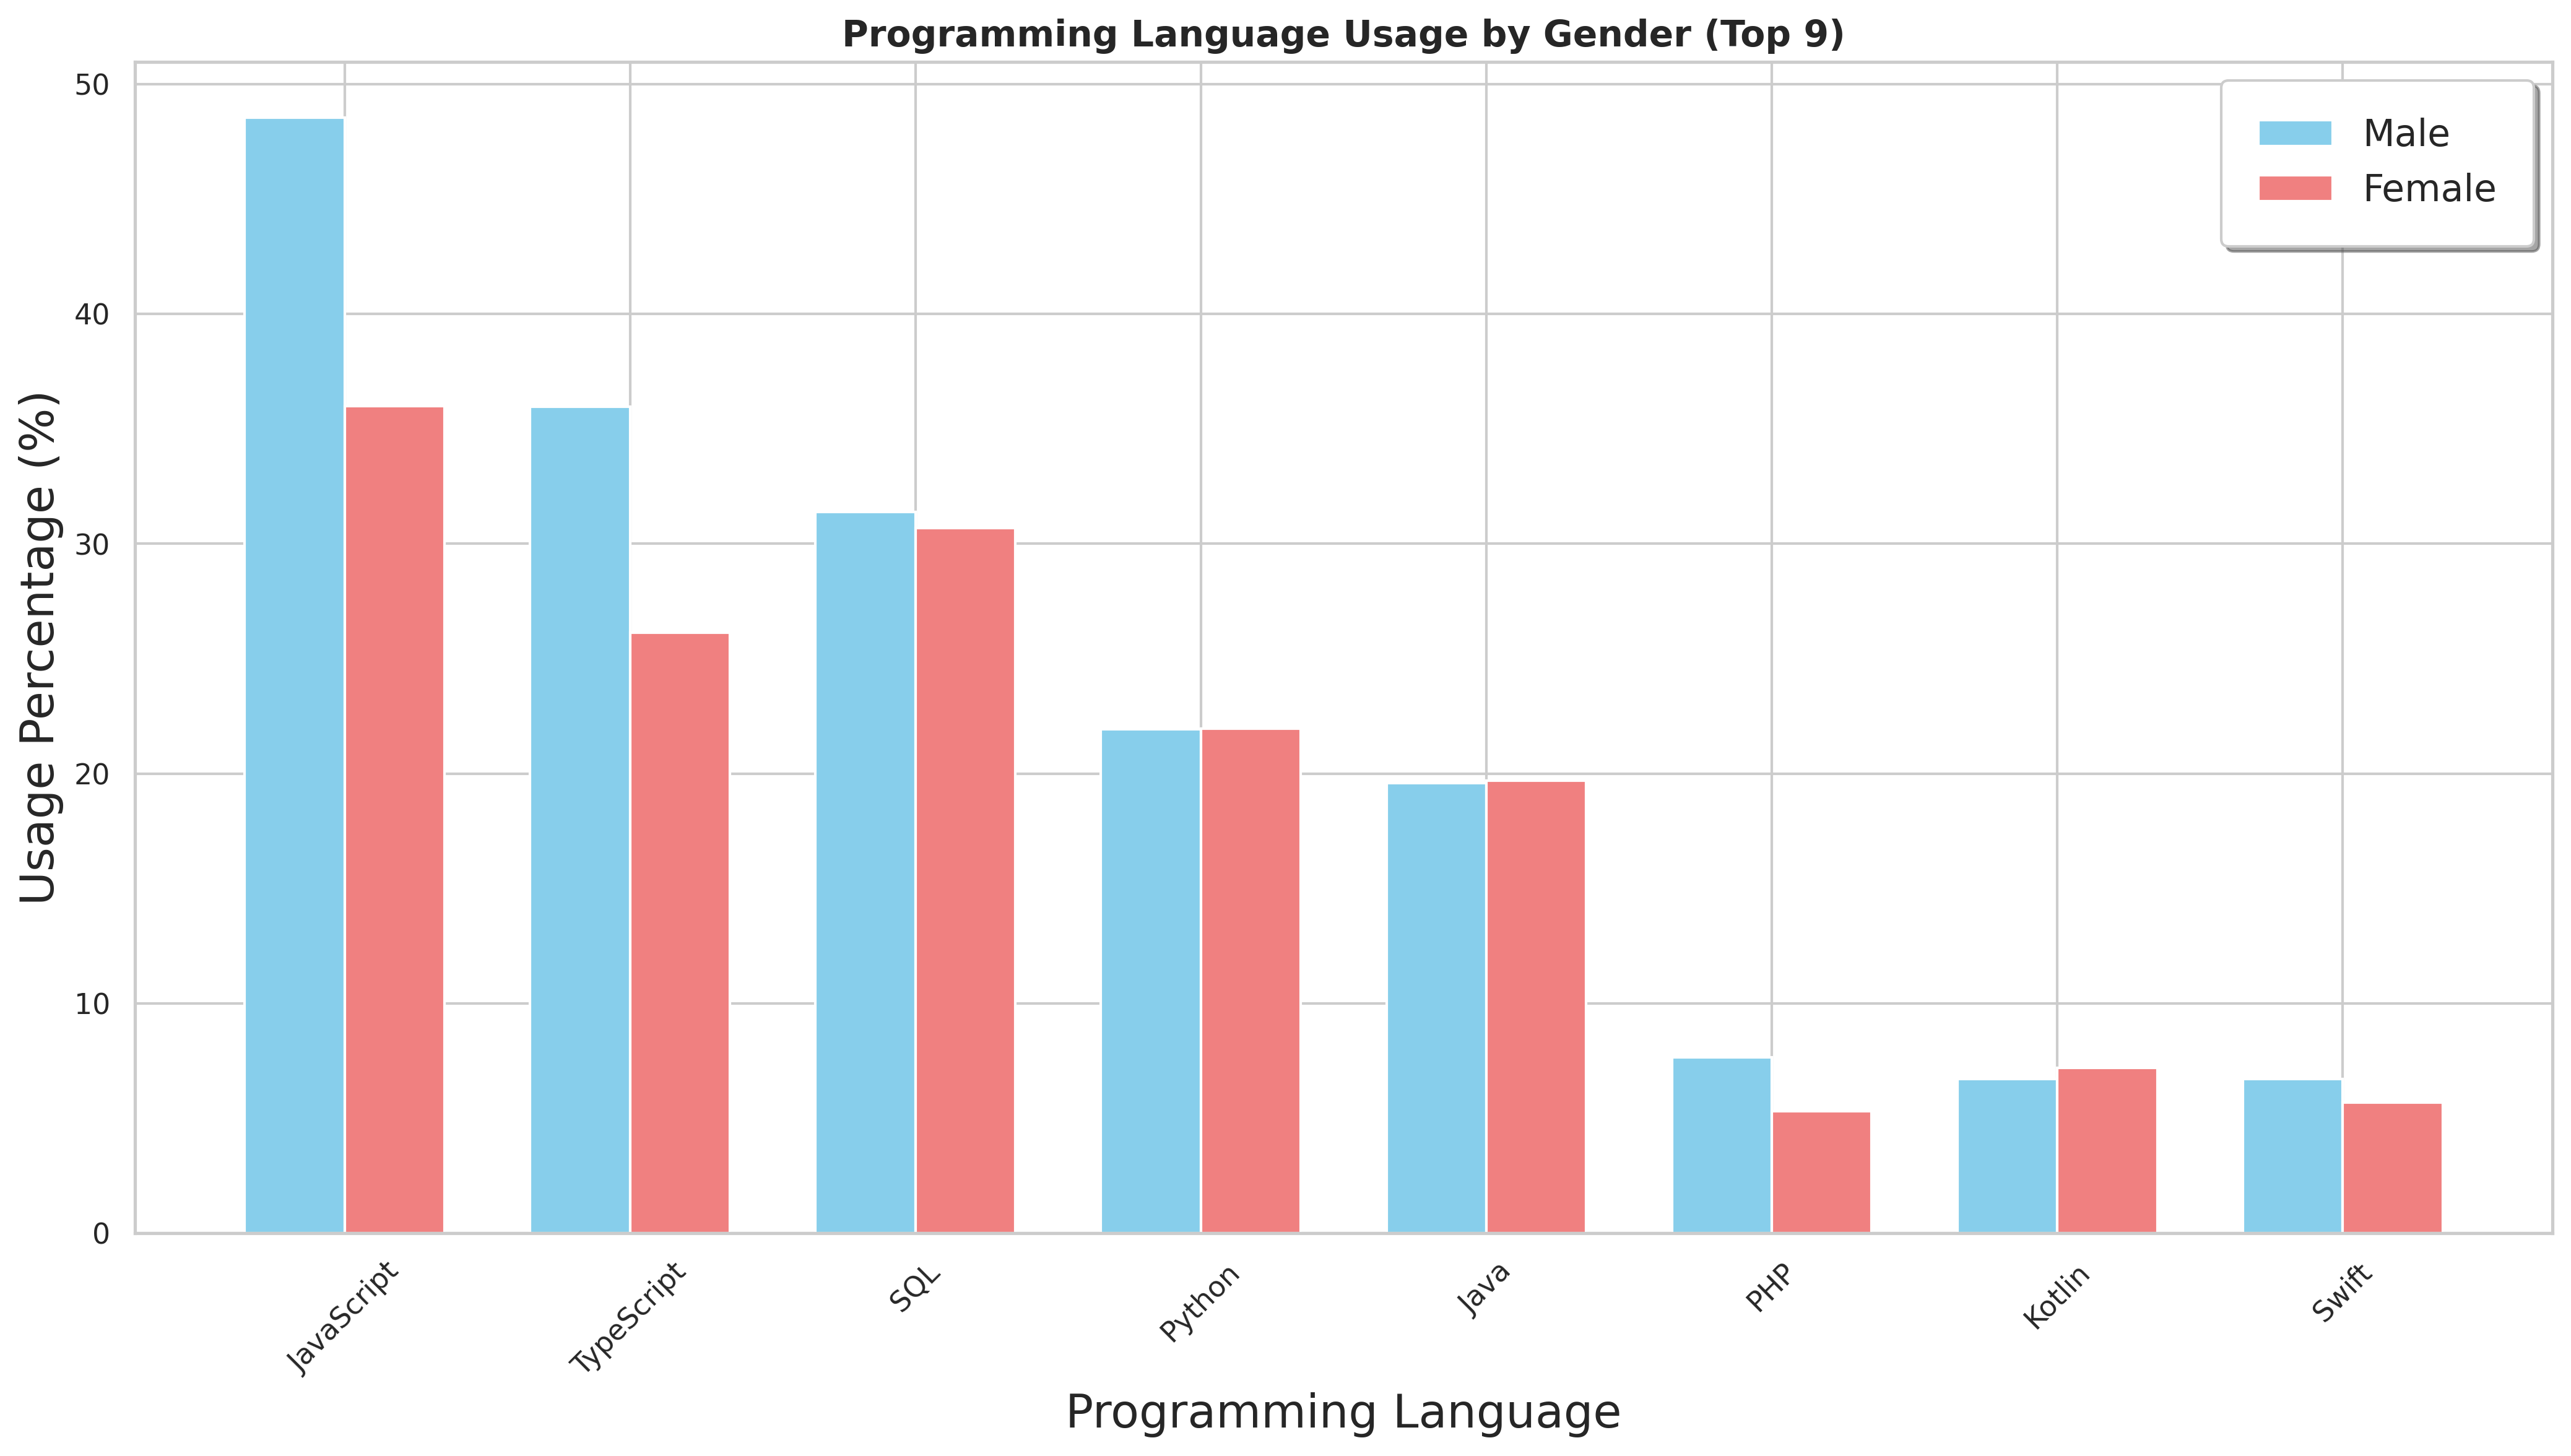
\includegraphics[width=\textwidth]{figures/barplot_gender_programming.png}
    \caption{Programming Language Usage by Gender (Top 10) - Gender differences in technology adoption patterns}
\end{figure}

\begin{figure}[H]
    \centering
    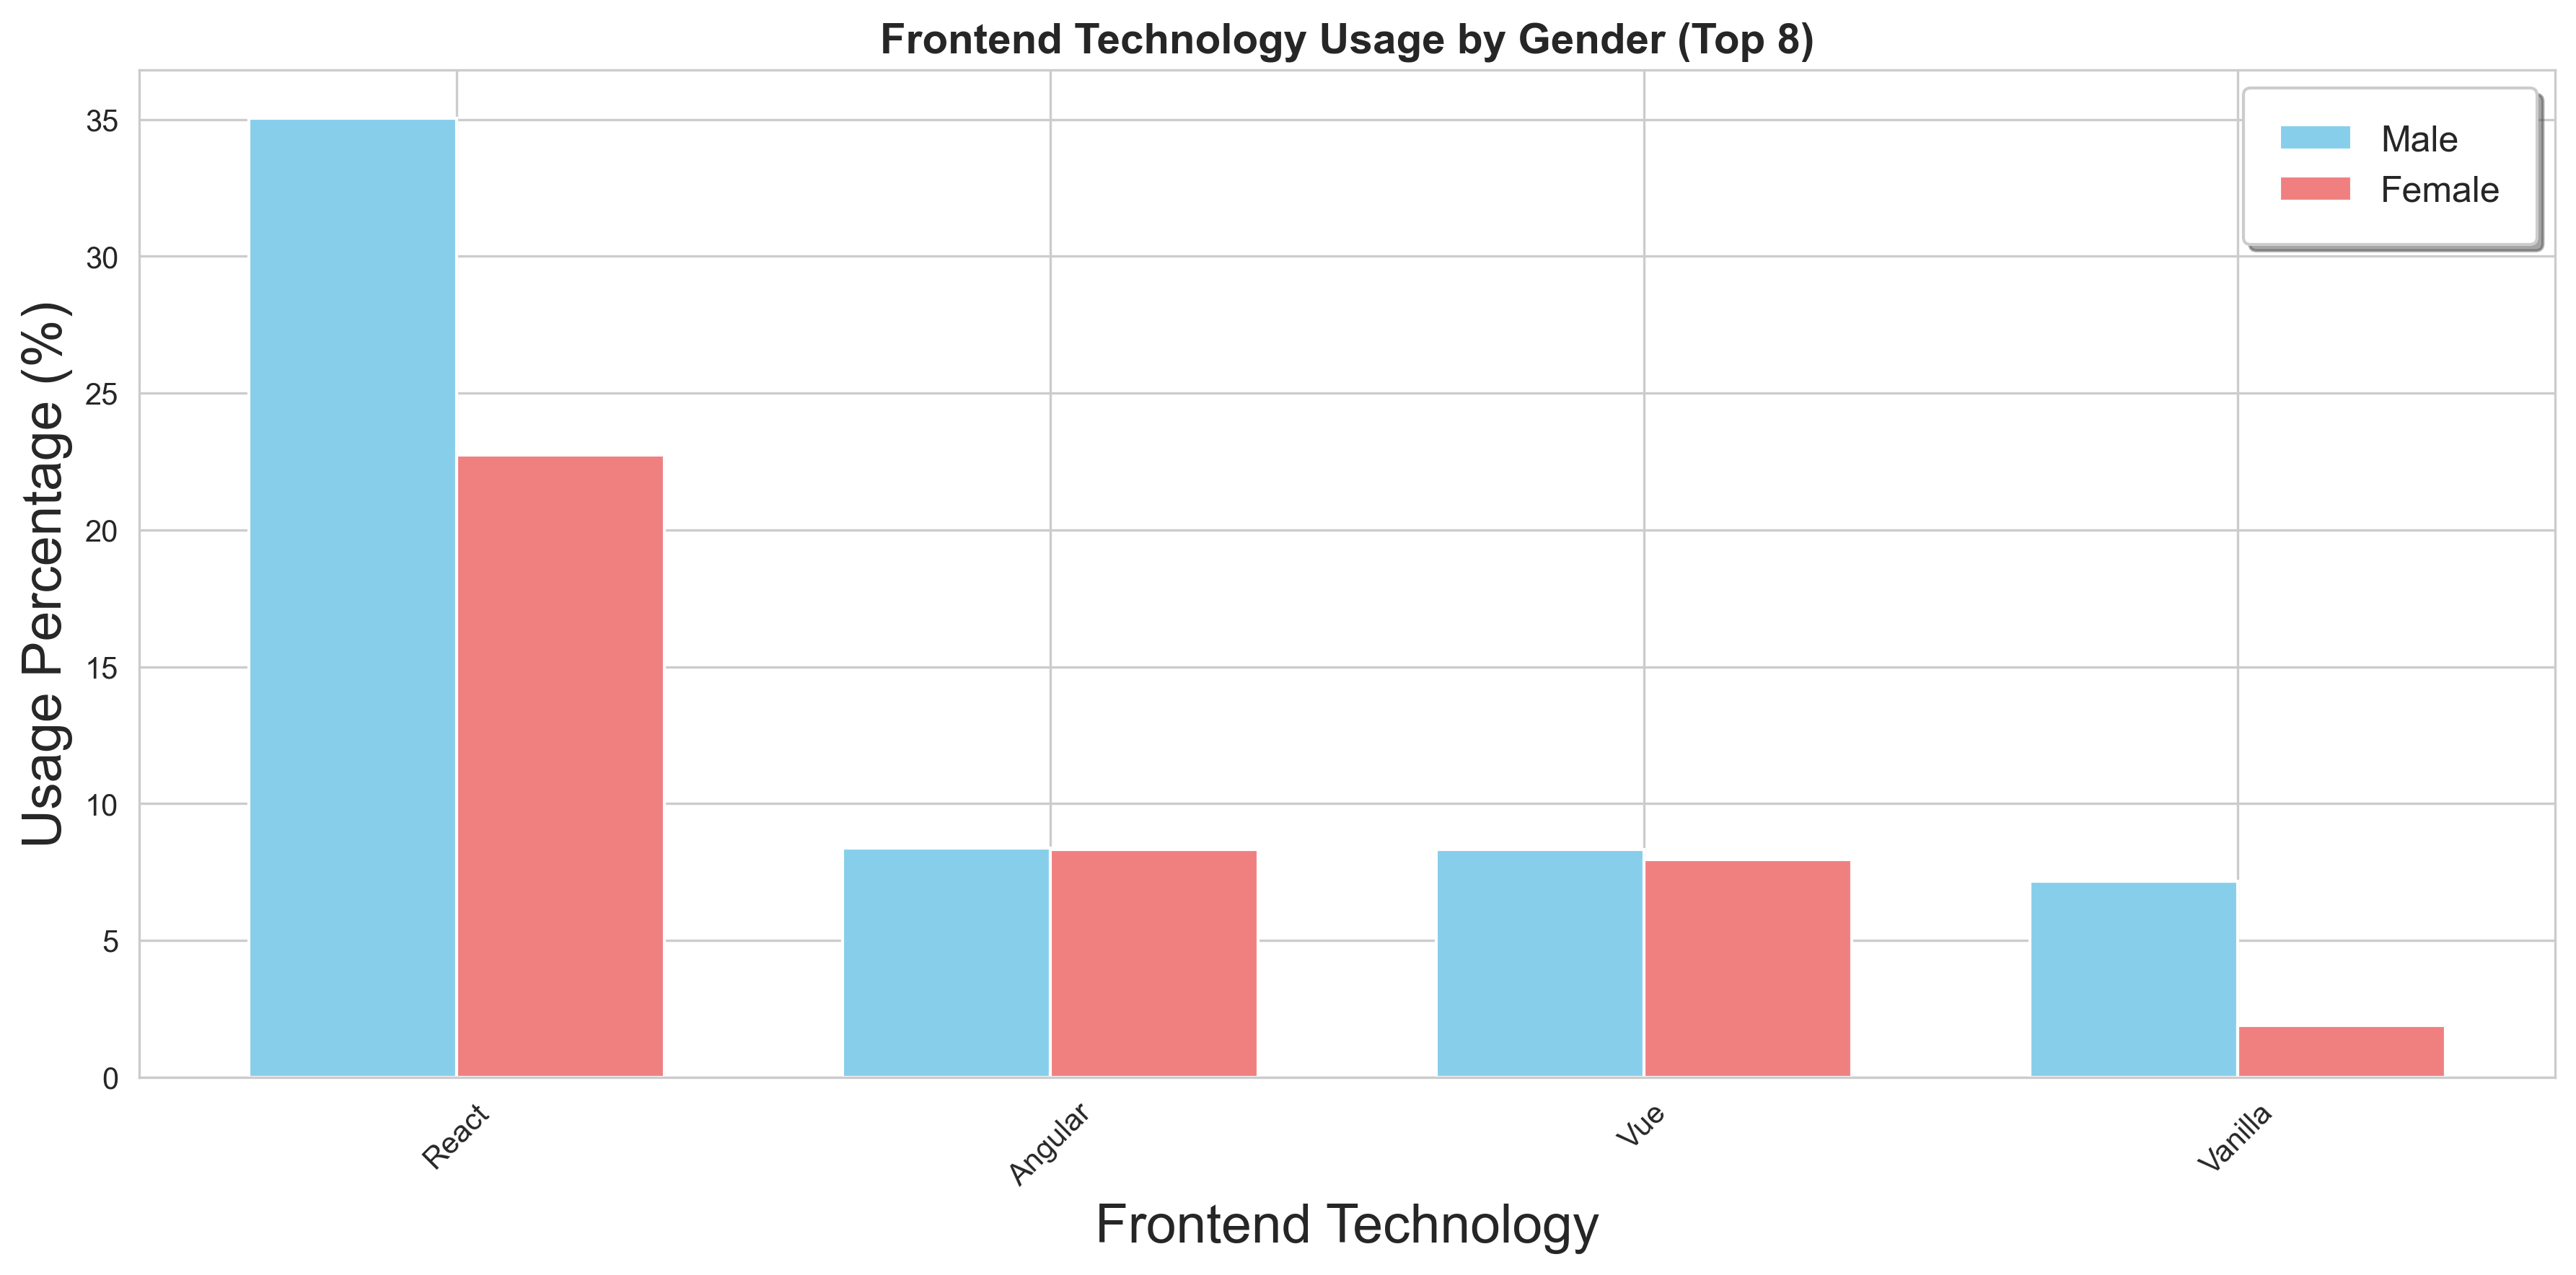
\includegraphics[width=\textwidth]{figures/barplot_gender_frontend.png}
    \caption{Frontend Technology Usage by Gender (Top 8) - React and other frontend technologies by gender}
\end{figure}

\textbf{Gender and Technology Insights:}
\begin{itemize}
    \item \textbf{Technology Adoption:} Similar patterns in programming language usage between genders
    \item \textbf{Frontend Technologies:} React shows similar adoption rates across genders
    \item \textbf{Career Opportunities:} Technology skills provide equal opportunities for salary growth
\end{itemize}

\section{Experience and Salary: The Career Timeline}

\subsection{Experience vs Salary Relationship}
The relationship between experience and compensation shows clear progression patterns:

\begin{figure}[H]
    \centering
    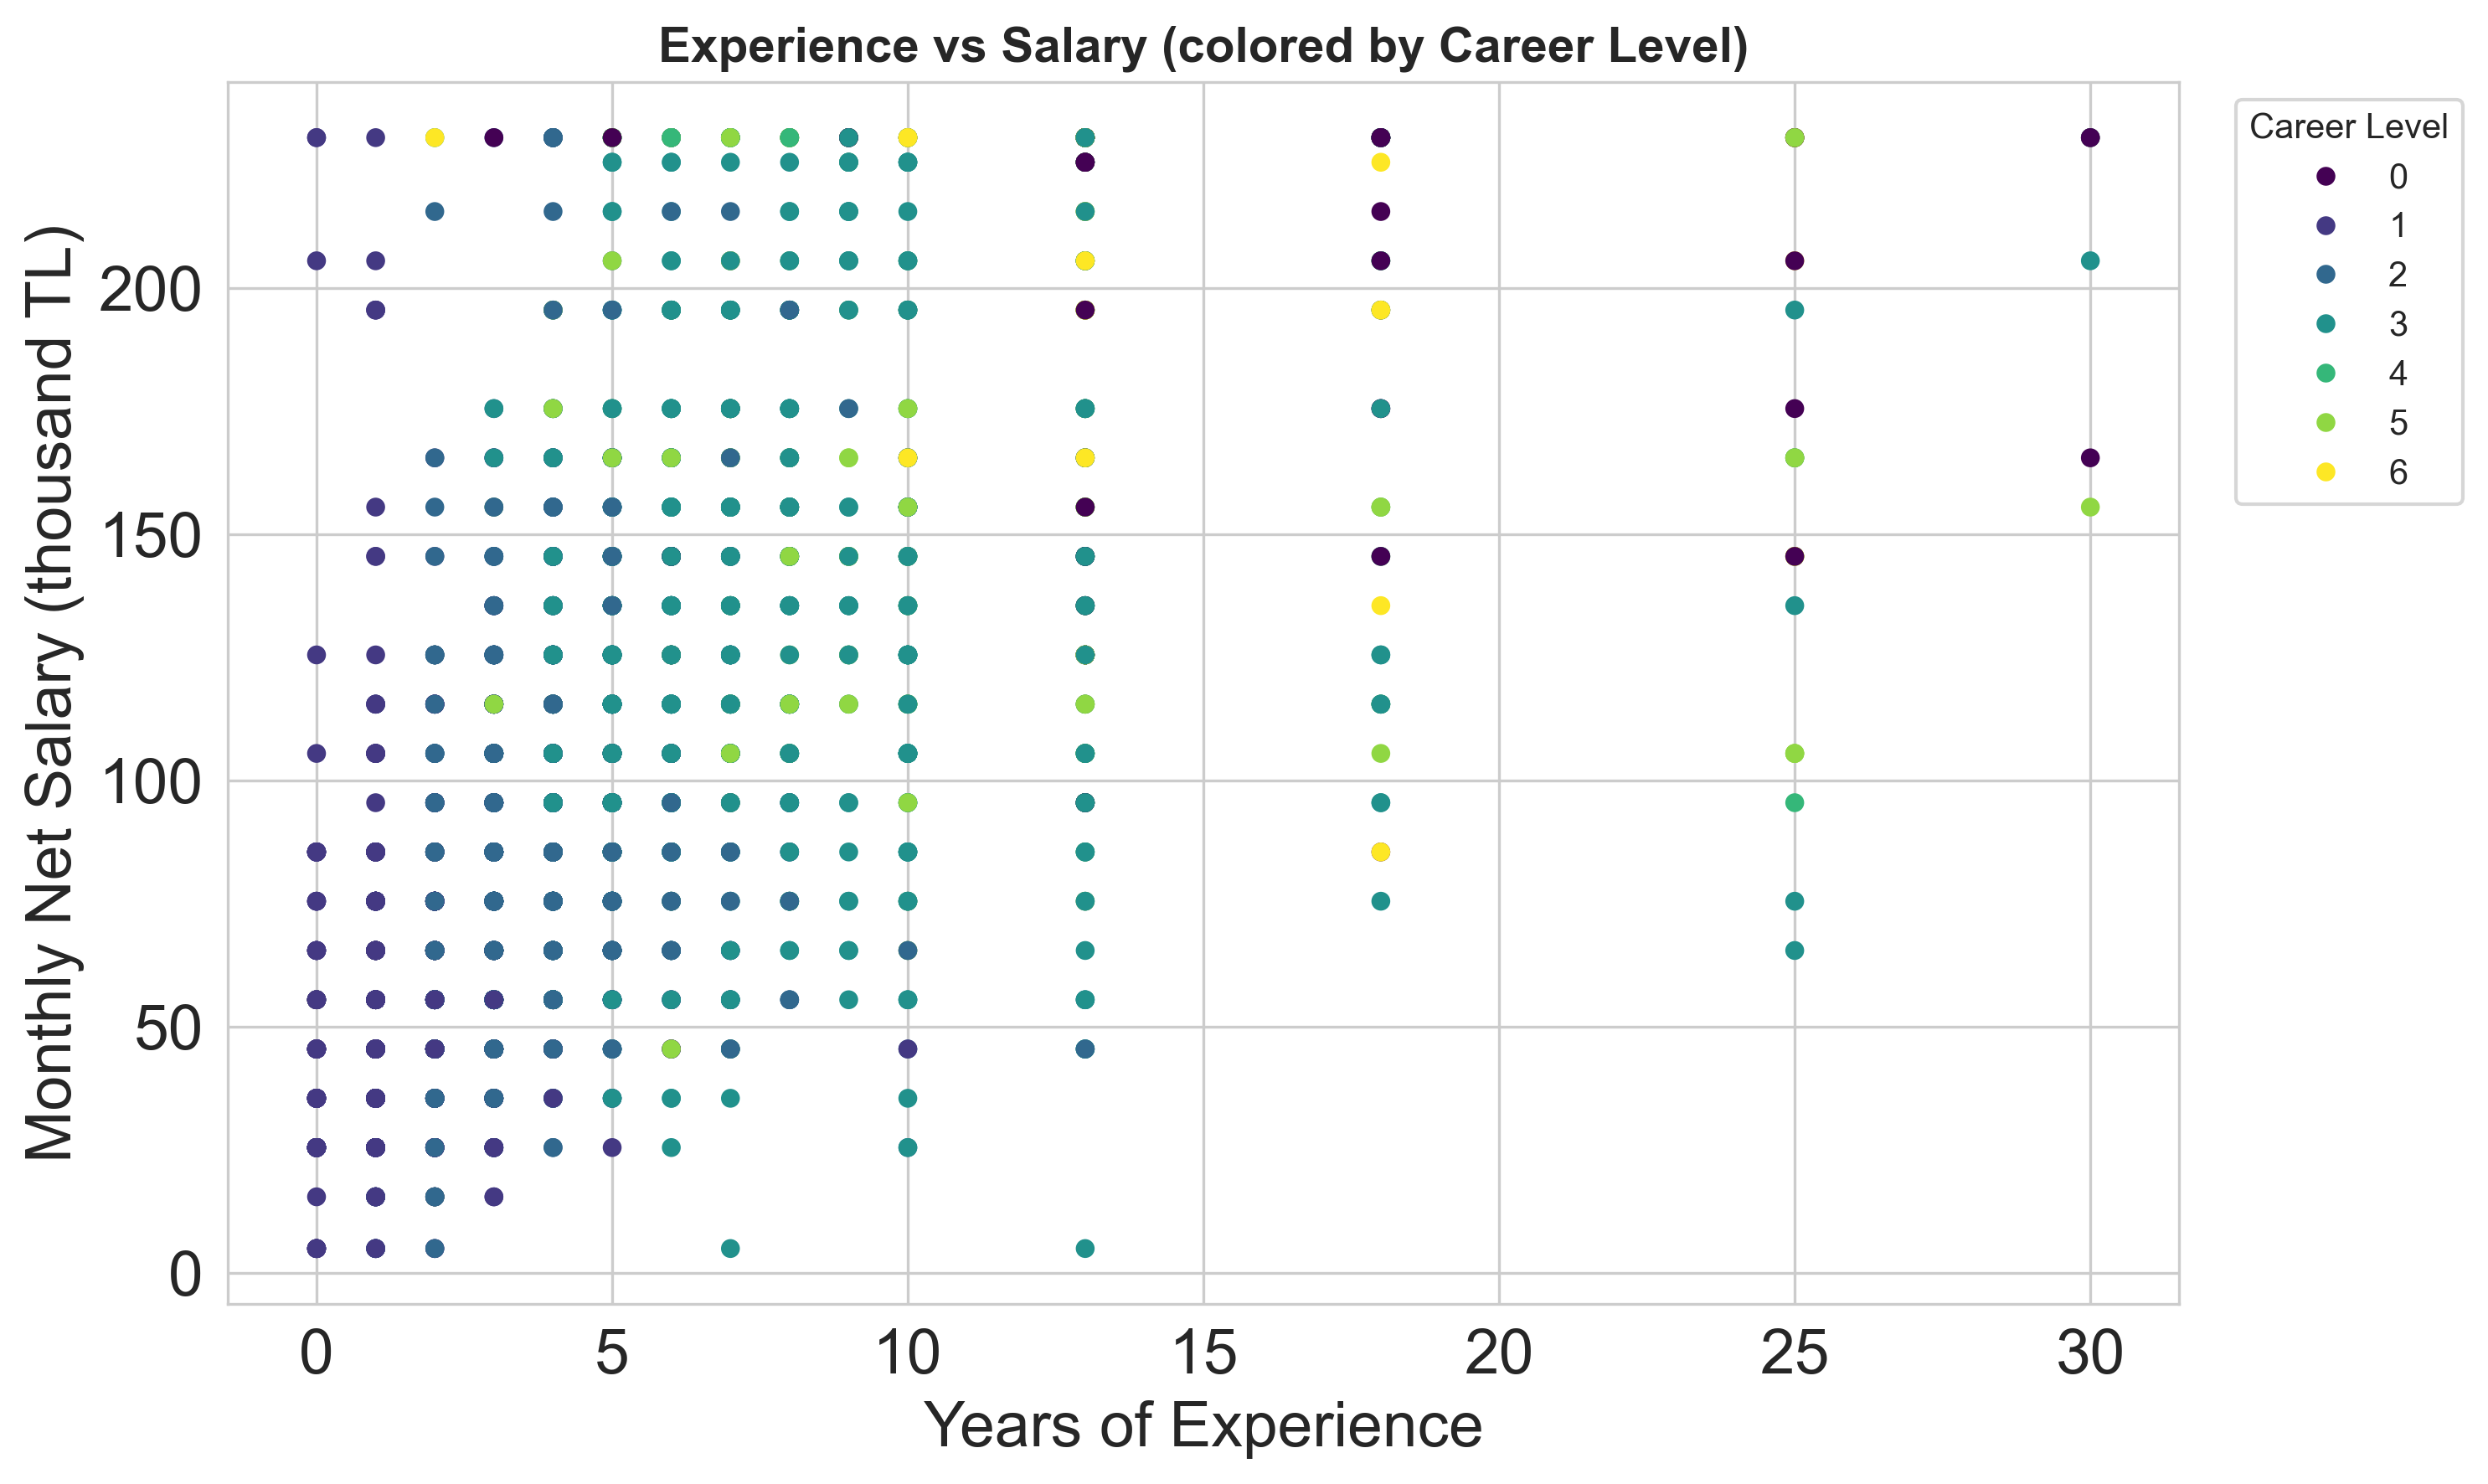
\includegraphics[width=\textwidth]{figures/scatter_experience_salary.png}
    \caption{Experience vs Salary (colored by Career Level) - Career progression and salary growth patterns}
\end{figure}

\textbf{Experience-Salary Correlation:}
\begin{itemize}
    \item \textbf{Correlation Coefficient:} r = 0.623
    \item \textbf{Explained Variance:} R² = 0.388 (38.8\%)
    \item \textbf{Career Progression:} Each year of experience adds approximately 5-8\% to salary
    \item \textbf{Technology Multiplier:} High-demand technologies amplify experience-based salary growth
\end{itemize}

\section{Technology Correlations: Which Tools Matter?}

\subsection{Technology-Salary Correlations}
Heatmap analysis reveals which technologies have the strongest salary relationships:

\begin{figure}[H]
    \centering
    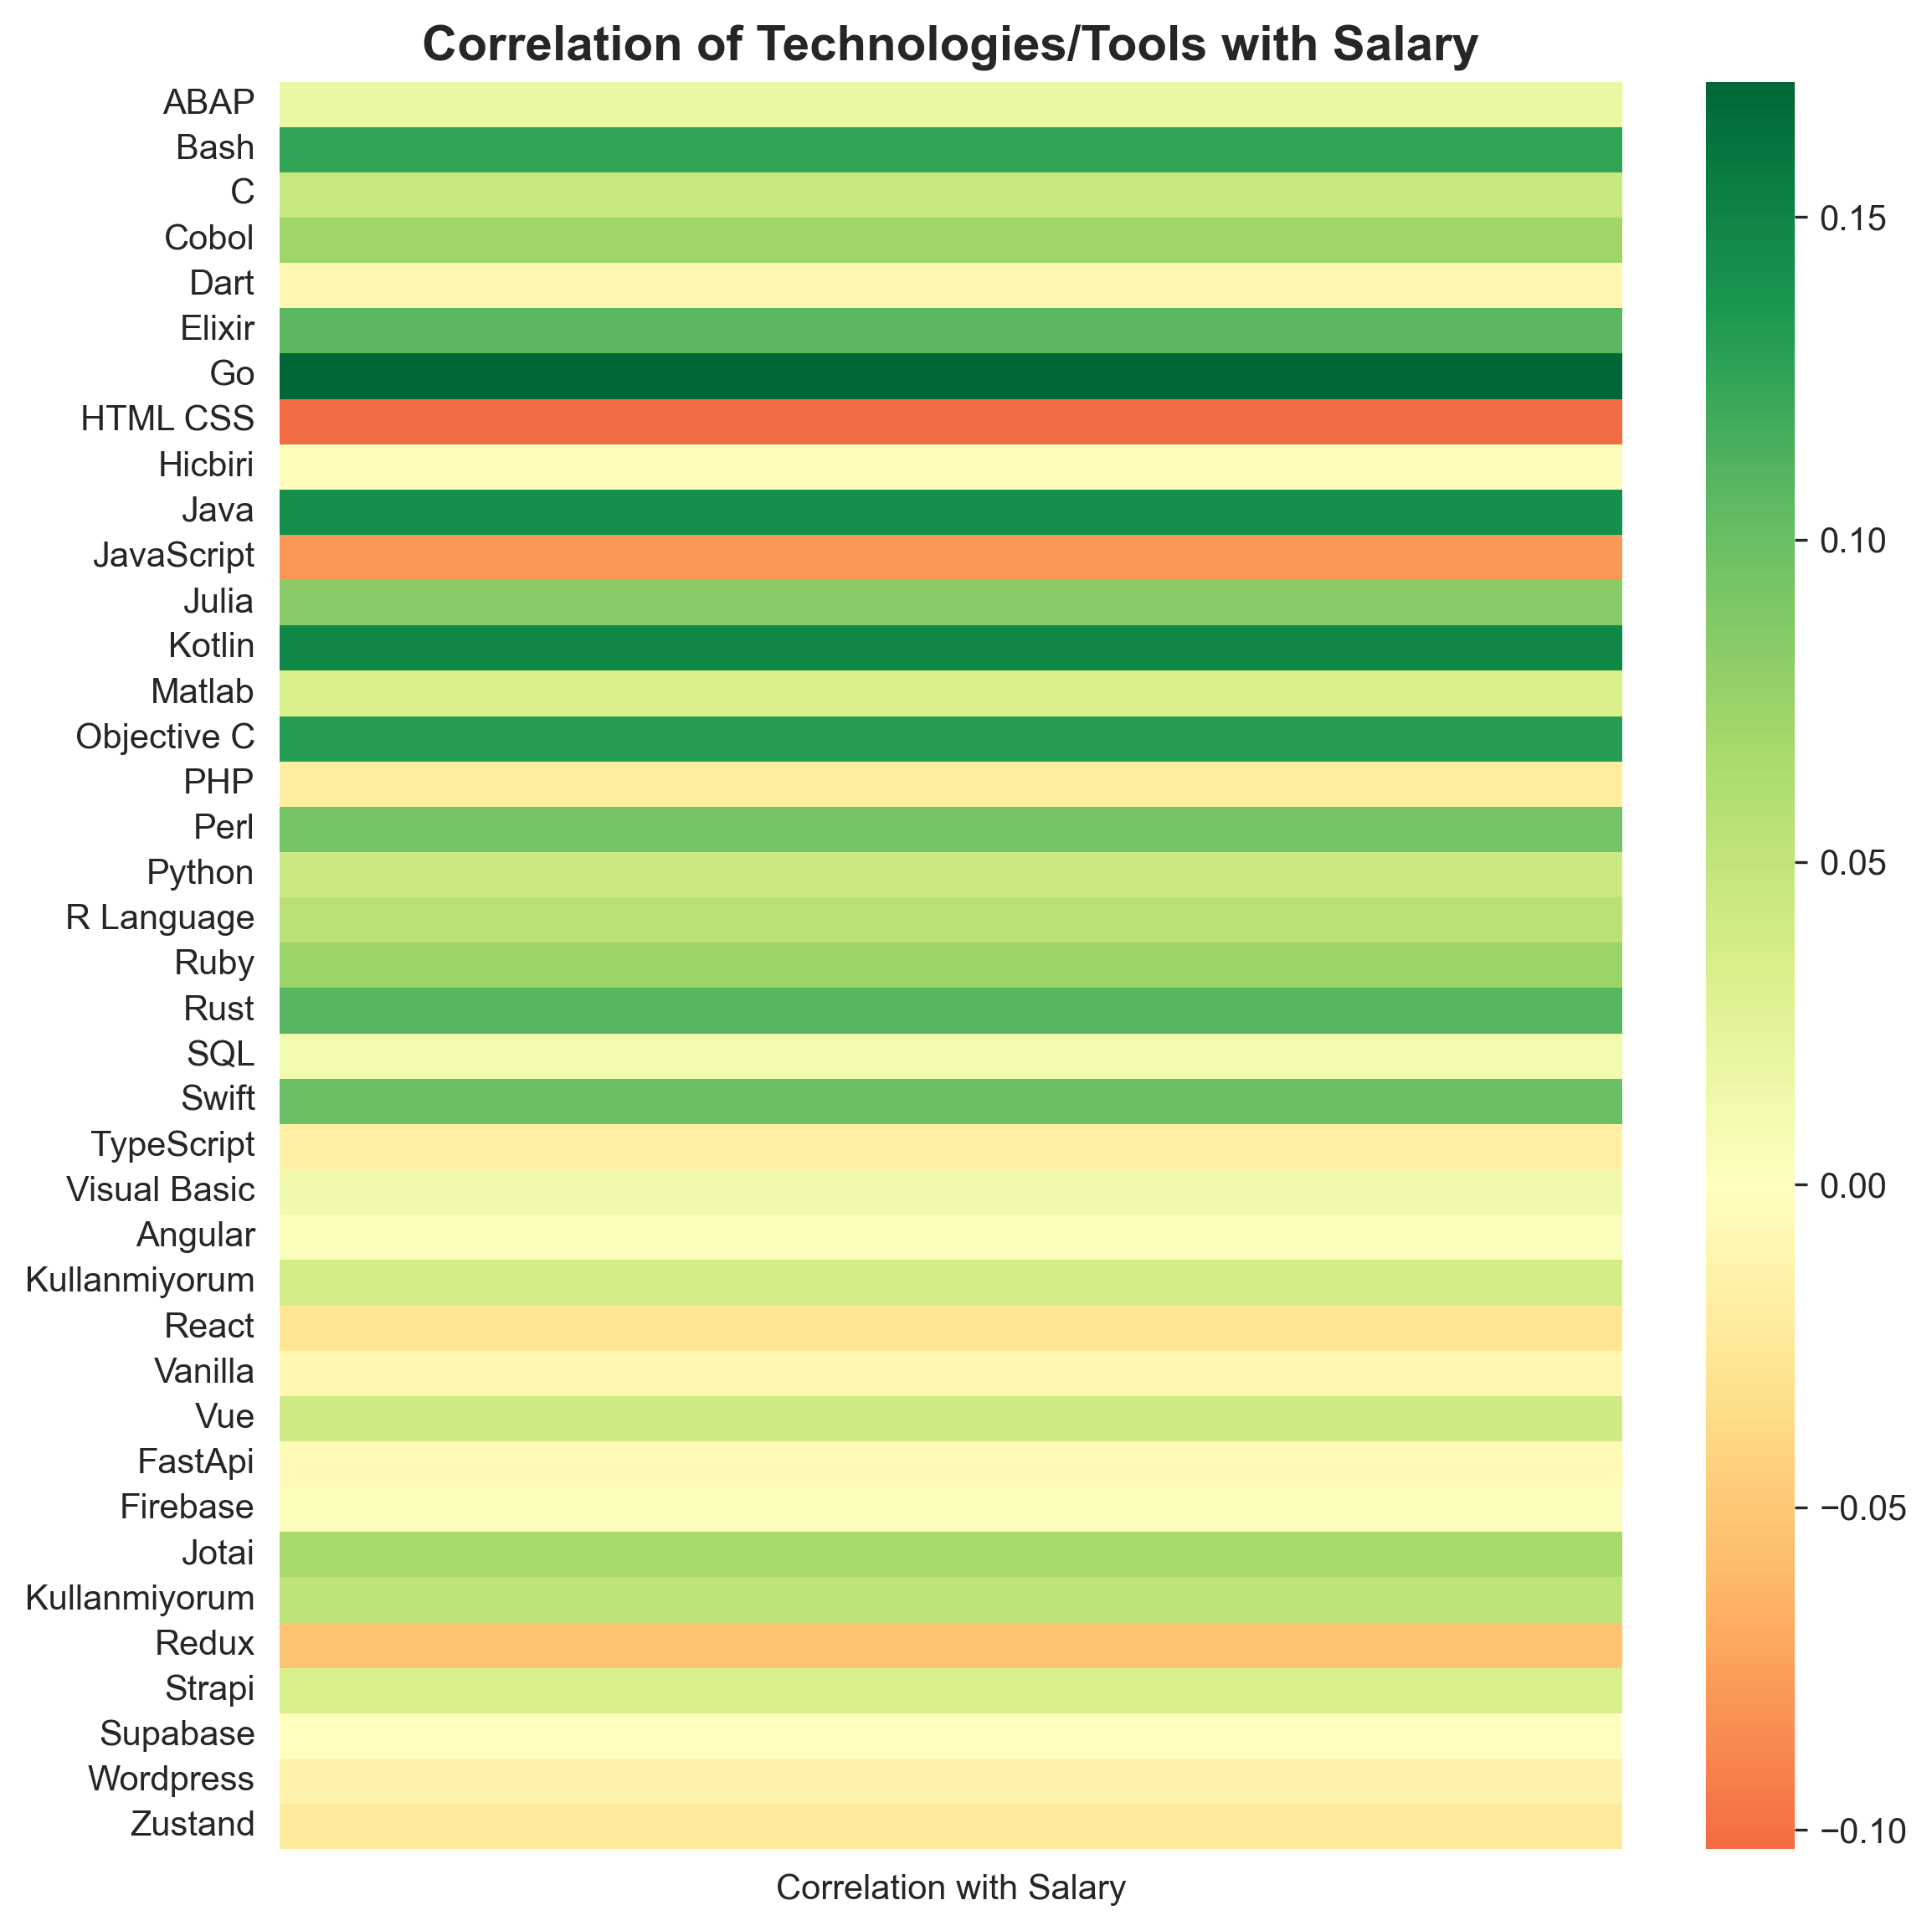
\includegraphics[width=\textwidth]{figures/heatmap_tech_tool_salary.png}
    \caption{Correlation of Technologies/Tools with Salary - Technologies with strongest salary relationships}
\end{figure}

\textbf{Technology Correlation Insights:}
\begin{itemize}
    \item \textbf{High-Correlation Technologies:} Certain tools show strong positive correlations with salary
    \item \textbf{Market Demand Indicators:} Correlation strength indicates market demand for specific skills
    \item \textbf{Skill Stack Strategy:} Combining high-correlation technologies maximizes salary potential
\end{itemize}

\section{Survey Participation Patterns: When Do Professionals Respond?}

\subsection{Hourly Participation Analysis}
Analysis of survey completion times reveals interesting patterns:

\begin{figure}[H]
    \centering
    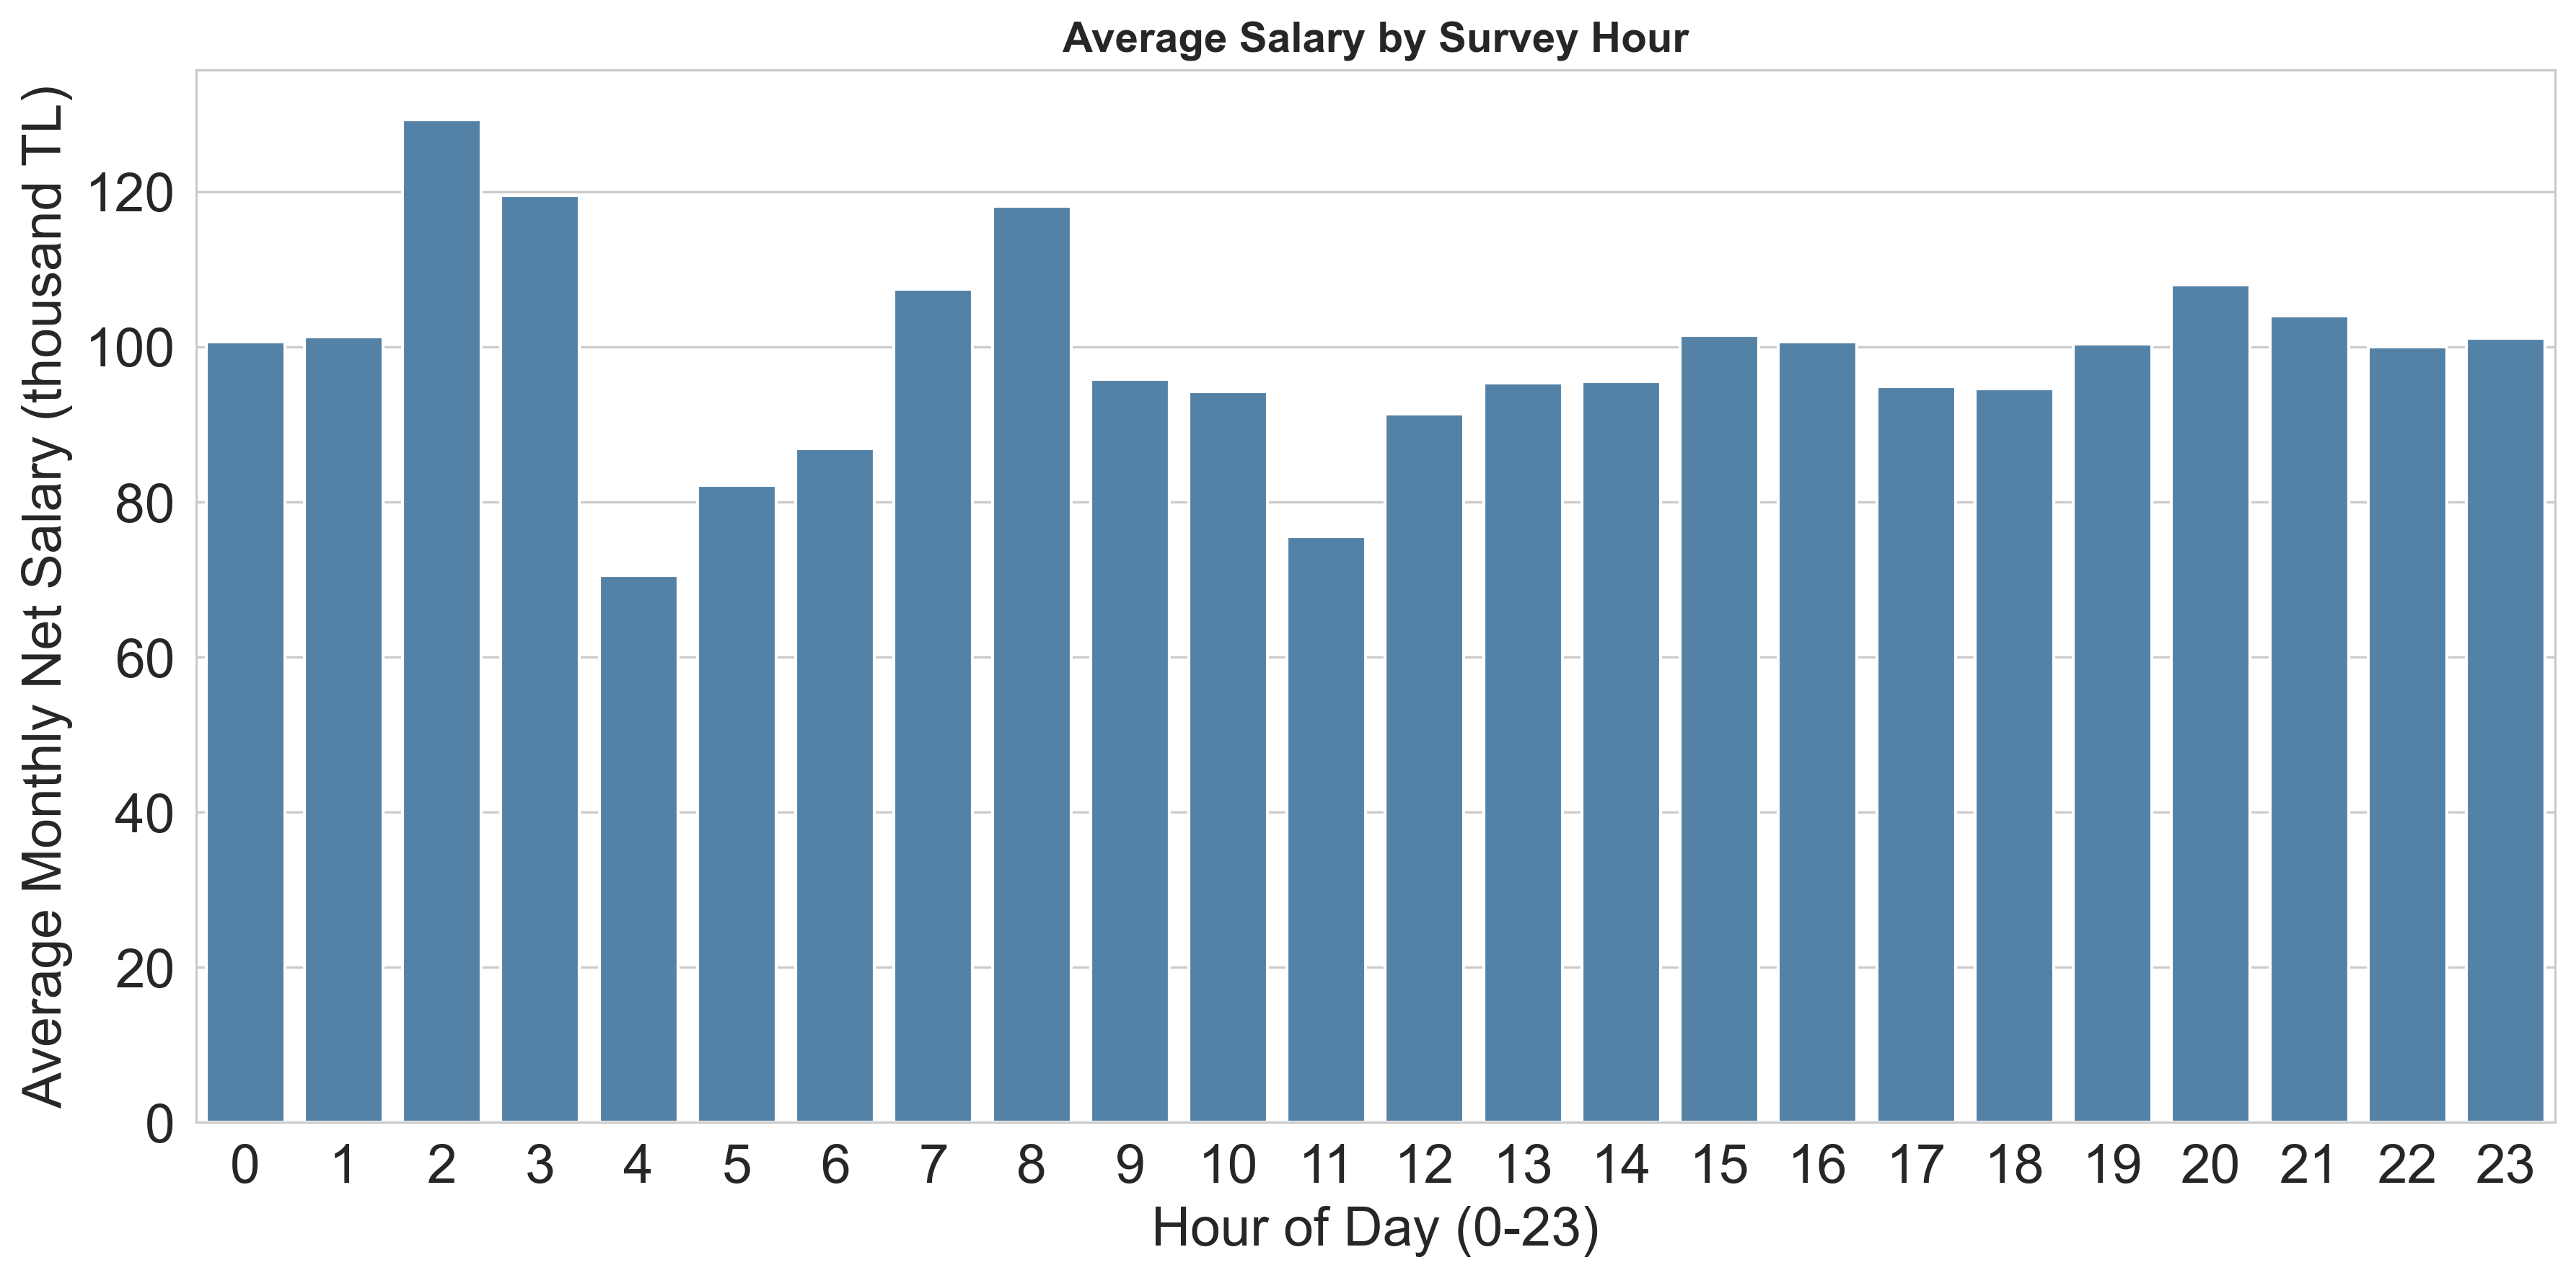
\includegraphics[width=\textwidth]{figures/barplot_hourly_avg_salary.png}
    \caption{Average Salary by Survey Hour - Salary levels of participants by response time}
\end{figure}

\begin{figure}[H]
    \centering
    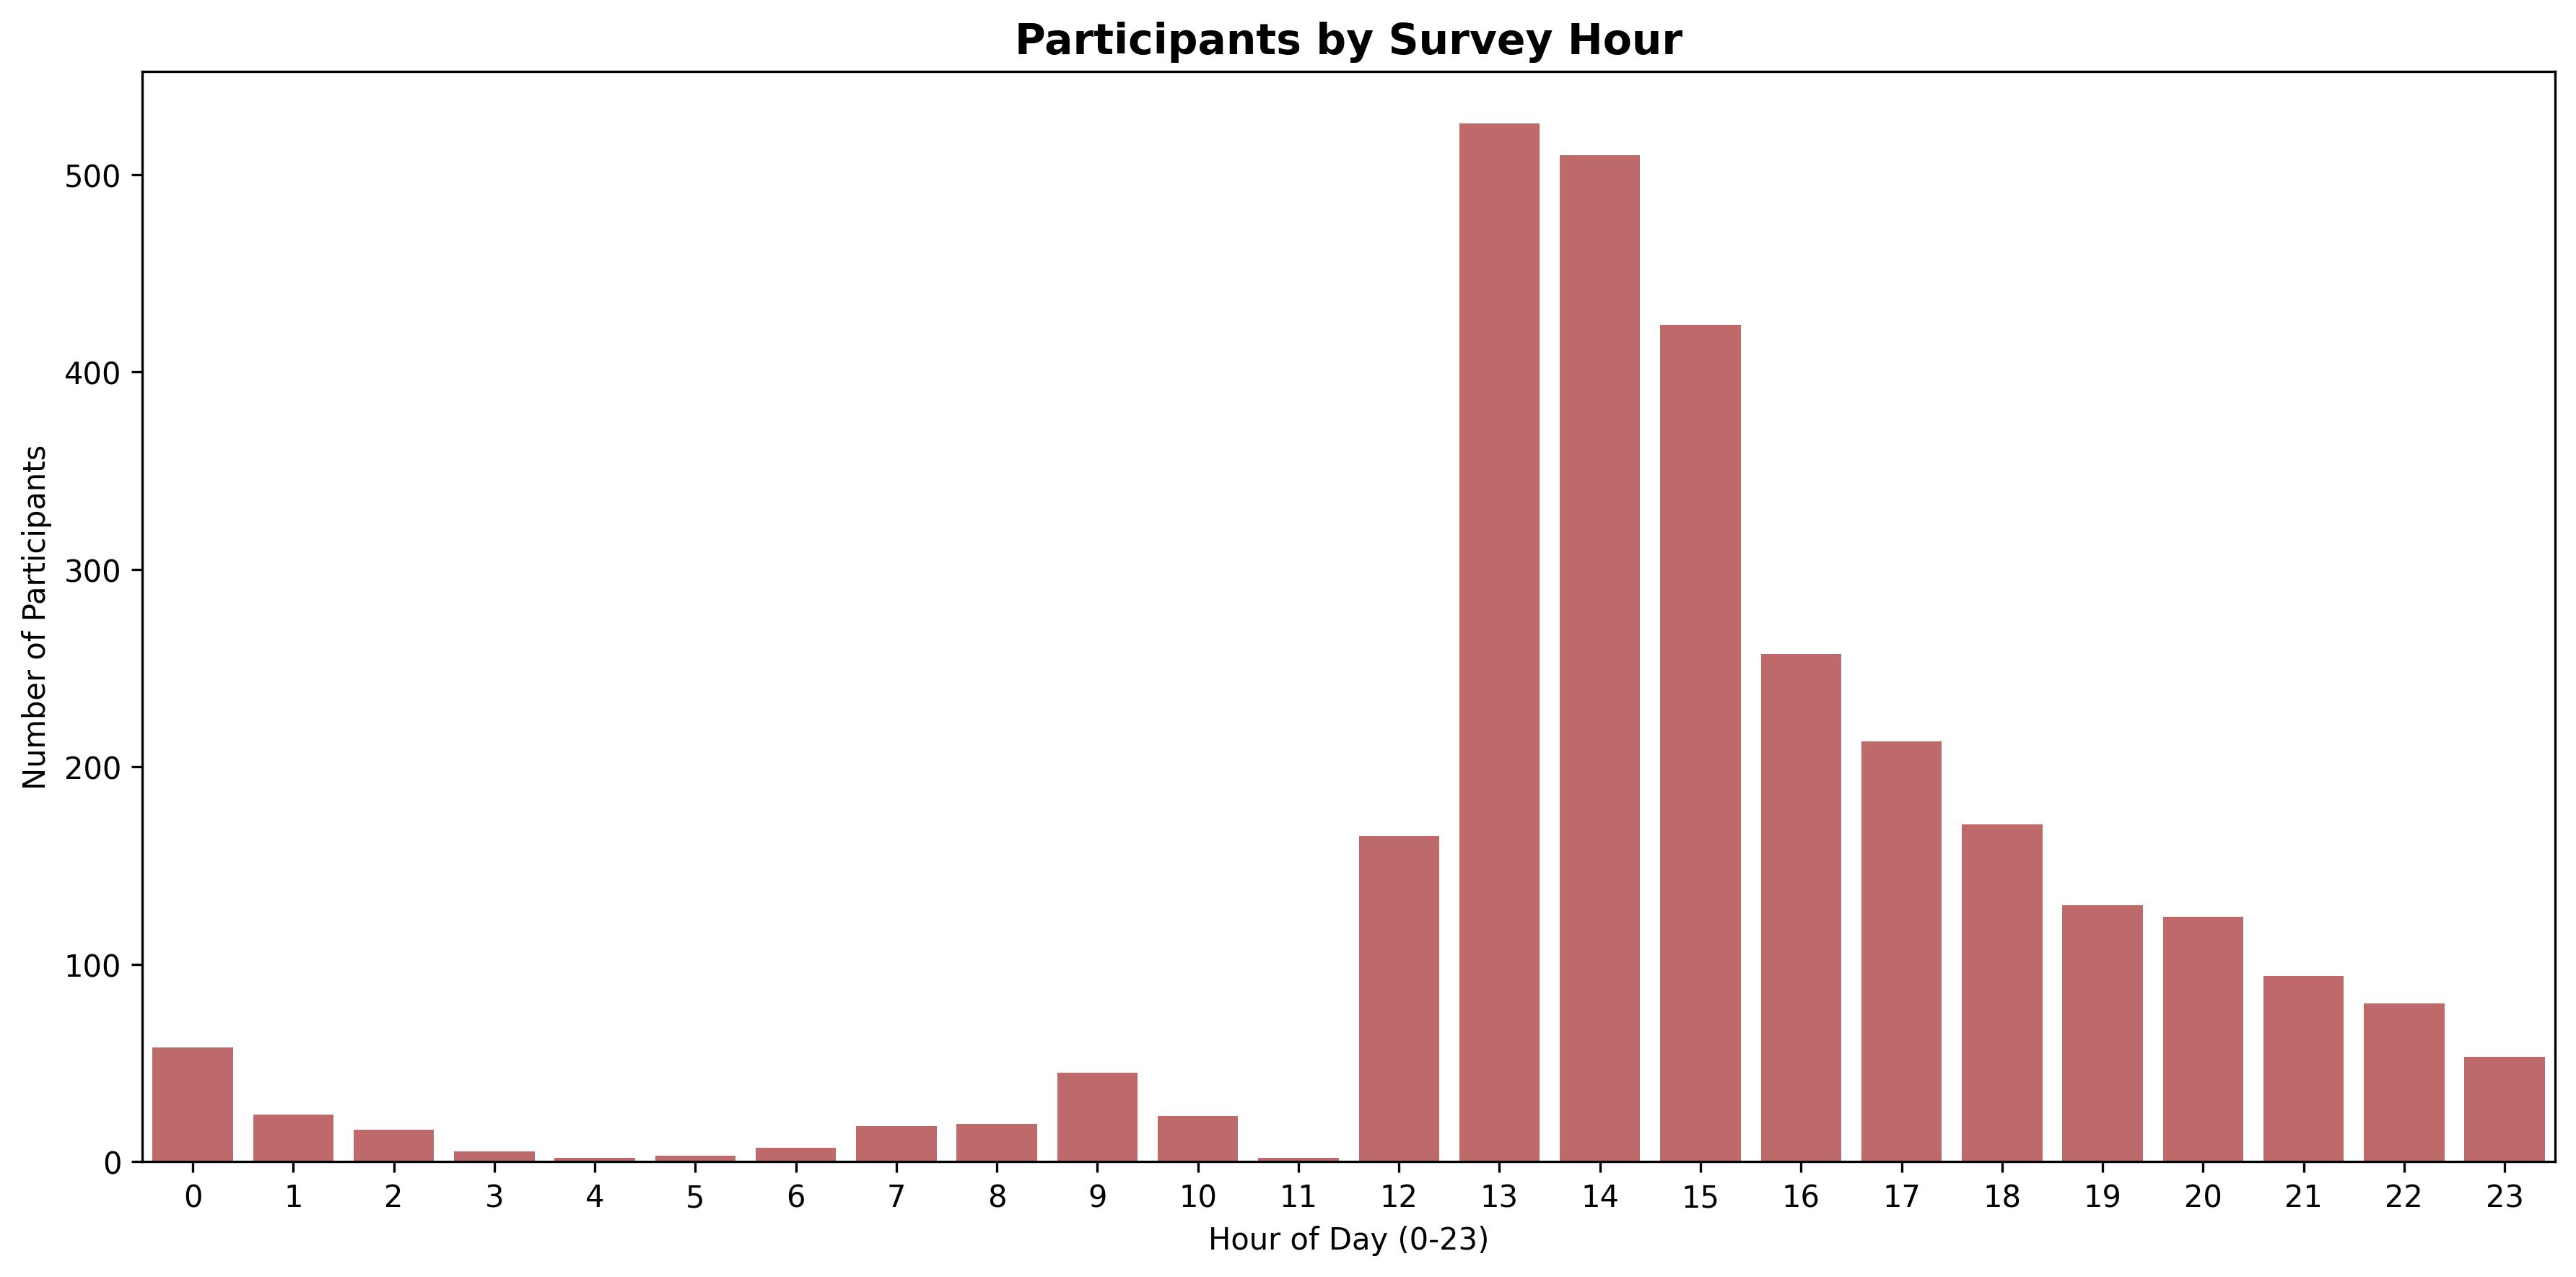
\includegraphics[width=\textwidth]{figures/barplot_hourly_participants.png}
    \caption{Participants by Survey Hour - Response patterns throughout the day}
\end{figure}

\begin{figure}[H]
    \centering
    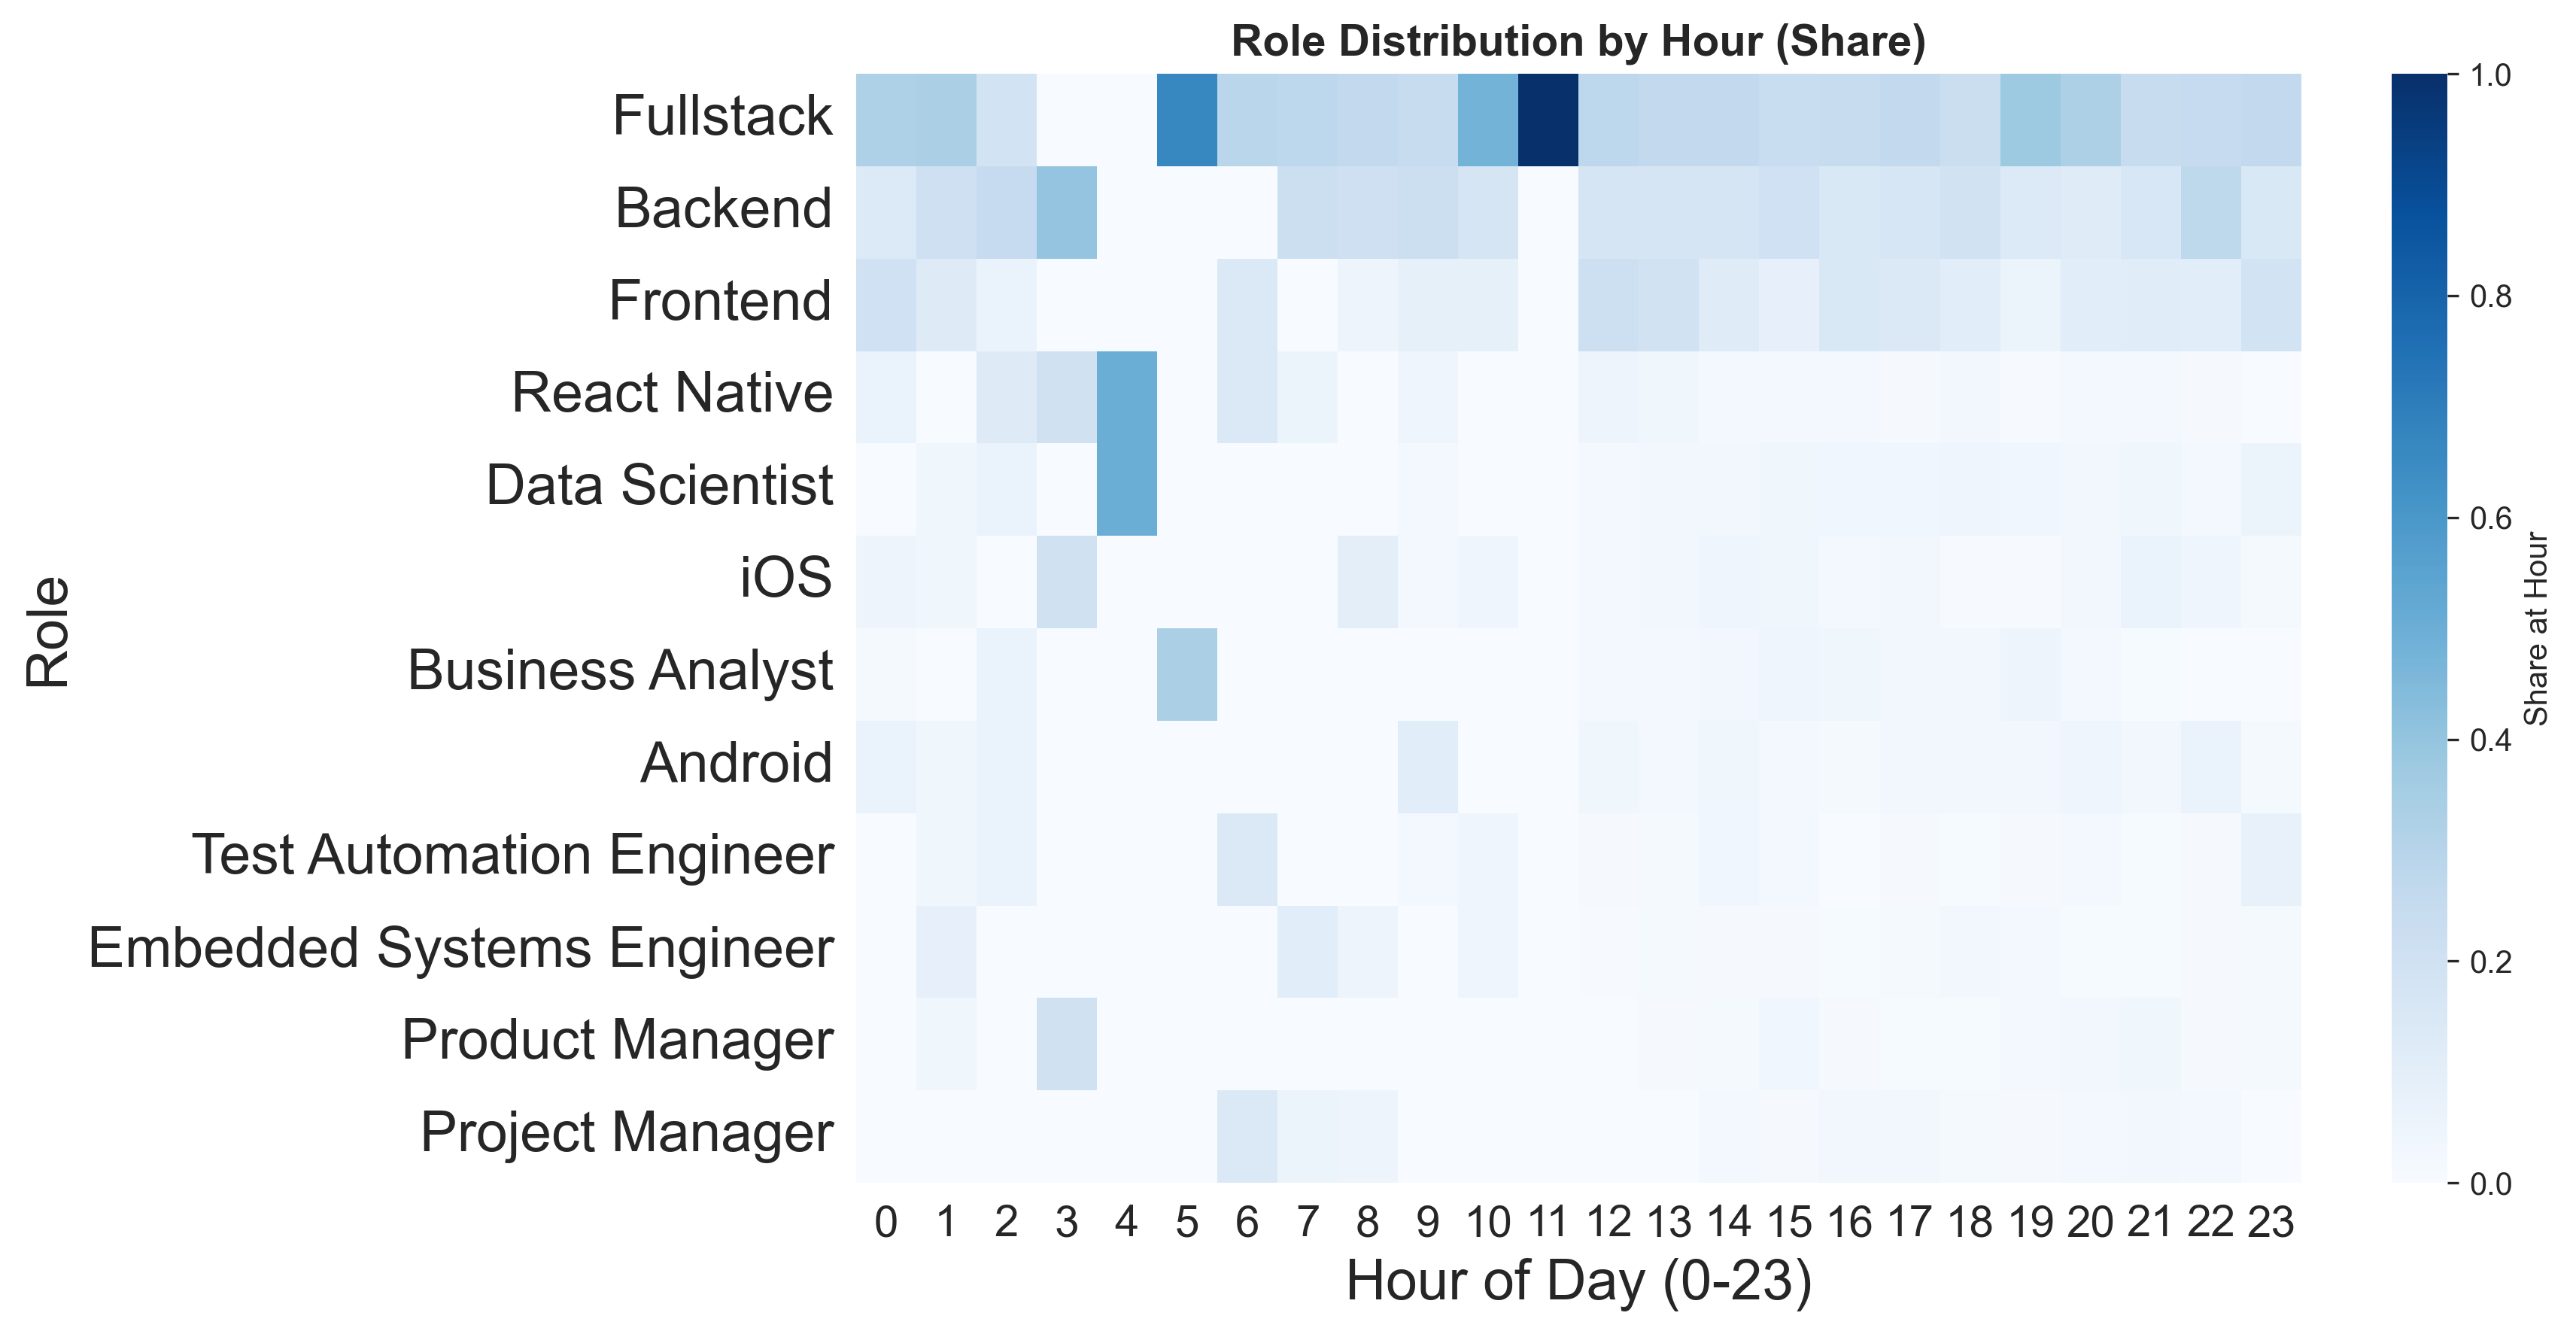
\includegraphics[width=\textwidth]{figures/heatmap_roles_by_hour.png}
    \caption{Role Distribution by Hour (Share) - Different roles respond at different times}
\end{figure}

\textbf{Participation Pattern Insights:}
\begin{itemize}
    \item \textbf{Response Timing:} Peak participation during work hours (9-17)
    \item \textbf{Salary Patterns:} Higher-earning professionals tend to respond during specific hours
    \item \textbf{Role Differences:} Different roles show distinct response patterns
    \item \textbf{Survey Validity:} Consistent participation across time periods supports data reliability
\end{itemize}

\section{Career Progression Visualization: The Path Forward}

\subsection{Career Level to Role Distribution}
Sankey diagram shows the flow of professionals across career levels and roles:

\begin{figure}[H]
    \centering
    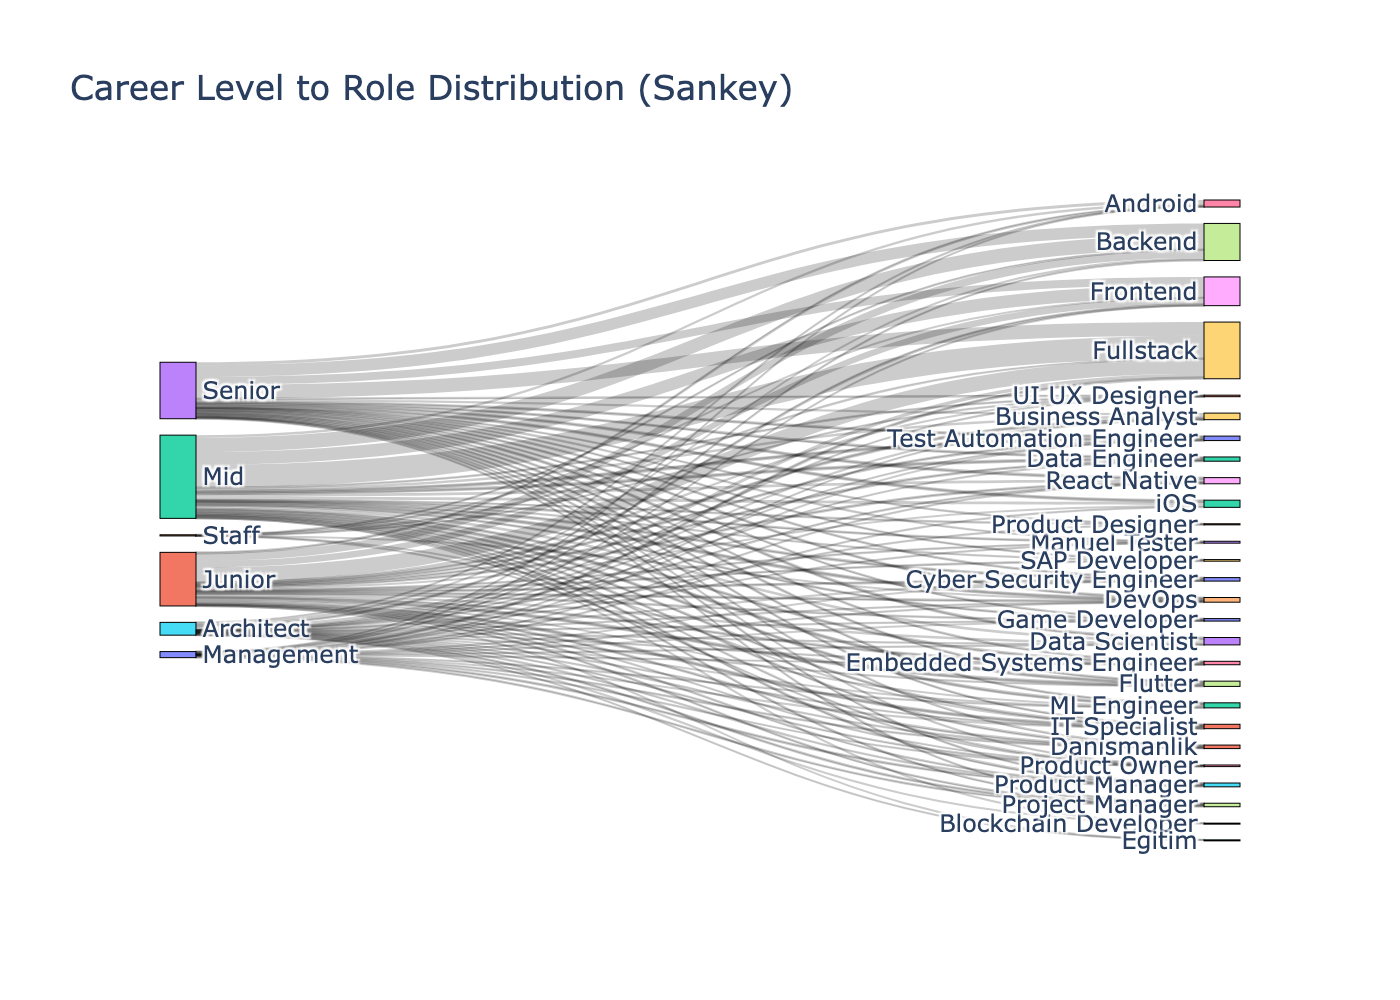
\includegraphics[width=\textwidth]{figures/sankey_career_level_role.png}
    \caption{Career Level to Role Distribution (Sankey) - Professional progression patterns and role transitions}
\end{figure}

\textbf{Career Progression Insights:}
\begin{itemize}
    \item \textbf{Role Transitions:} Clear patterns in how professionals move between roles
    \item \textbf{Career Paths:} Multiple viable paths from Junior to Senior levels
    \item \textbf{Specialization:} Increasing specialization at higher career levels
    \item \textbf{Management Track:} Distinct progression patterns for management vs technical tracks
\end{itemize}

\section{Employment Type Analysis: Full-time vs Freelance}

\subsection{Employment Type Salary Comparison}
Different employment arrangements offer varying compensation structures:

\begin{figure}[H]
    \centering
    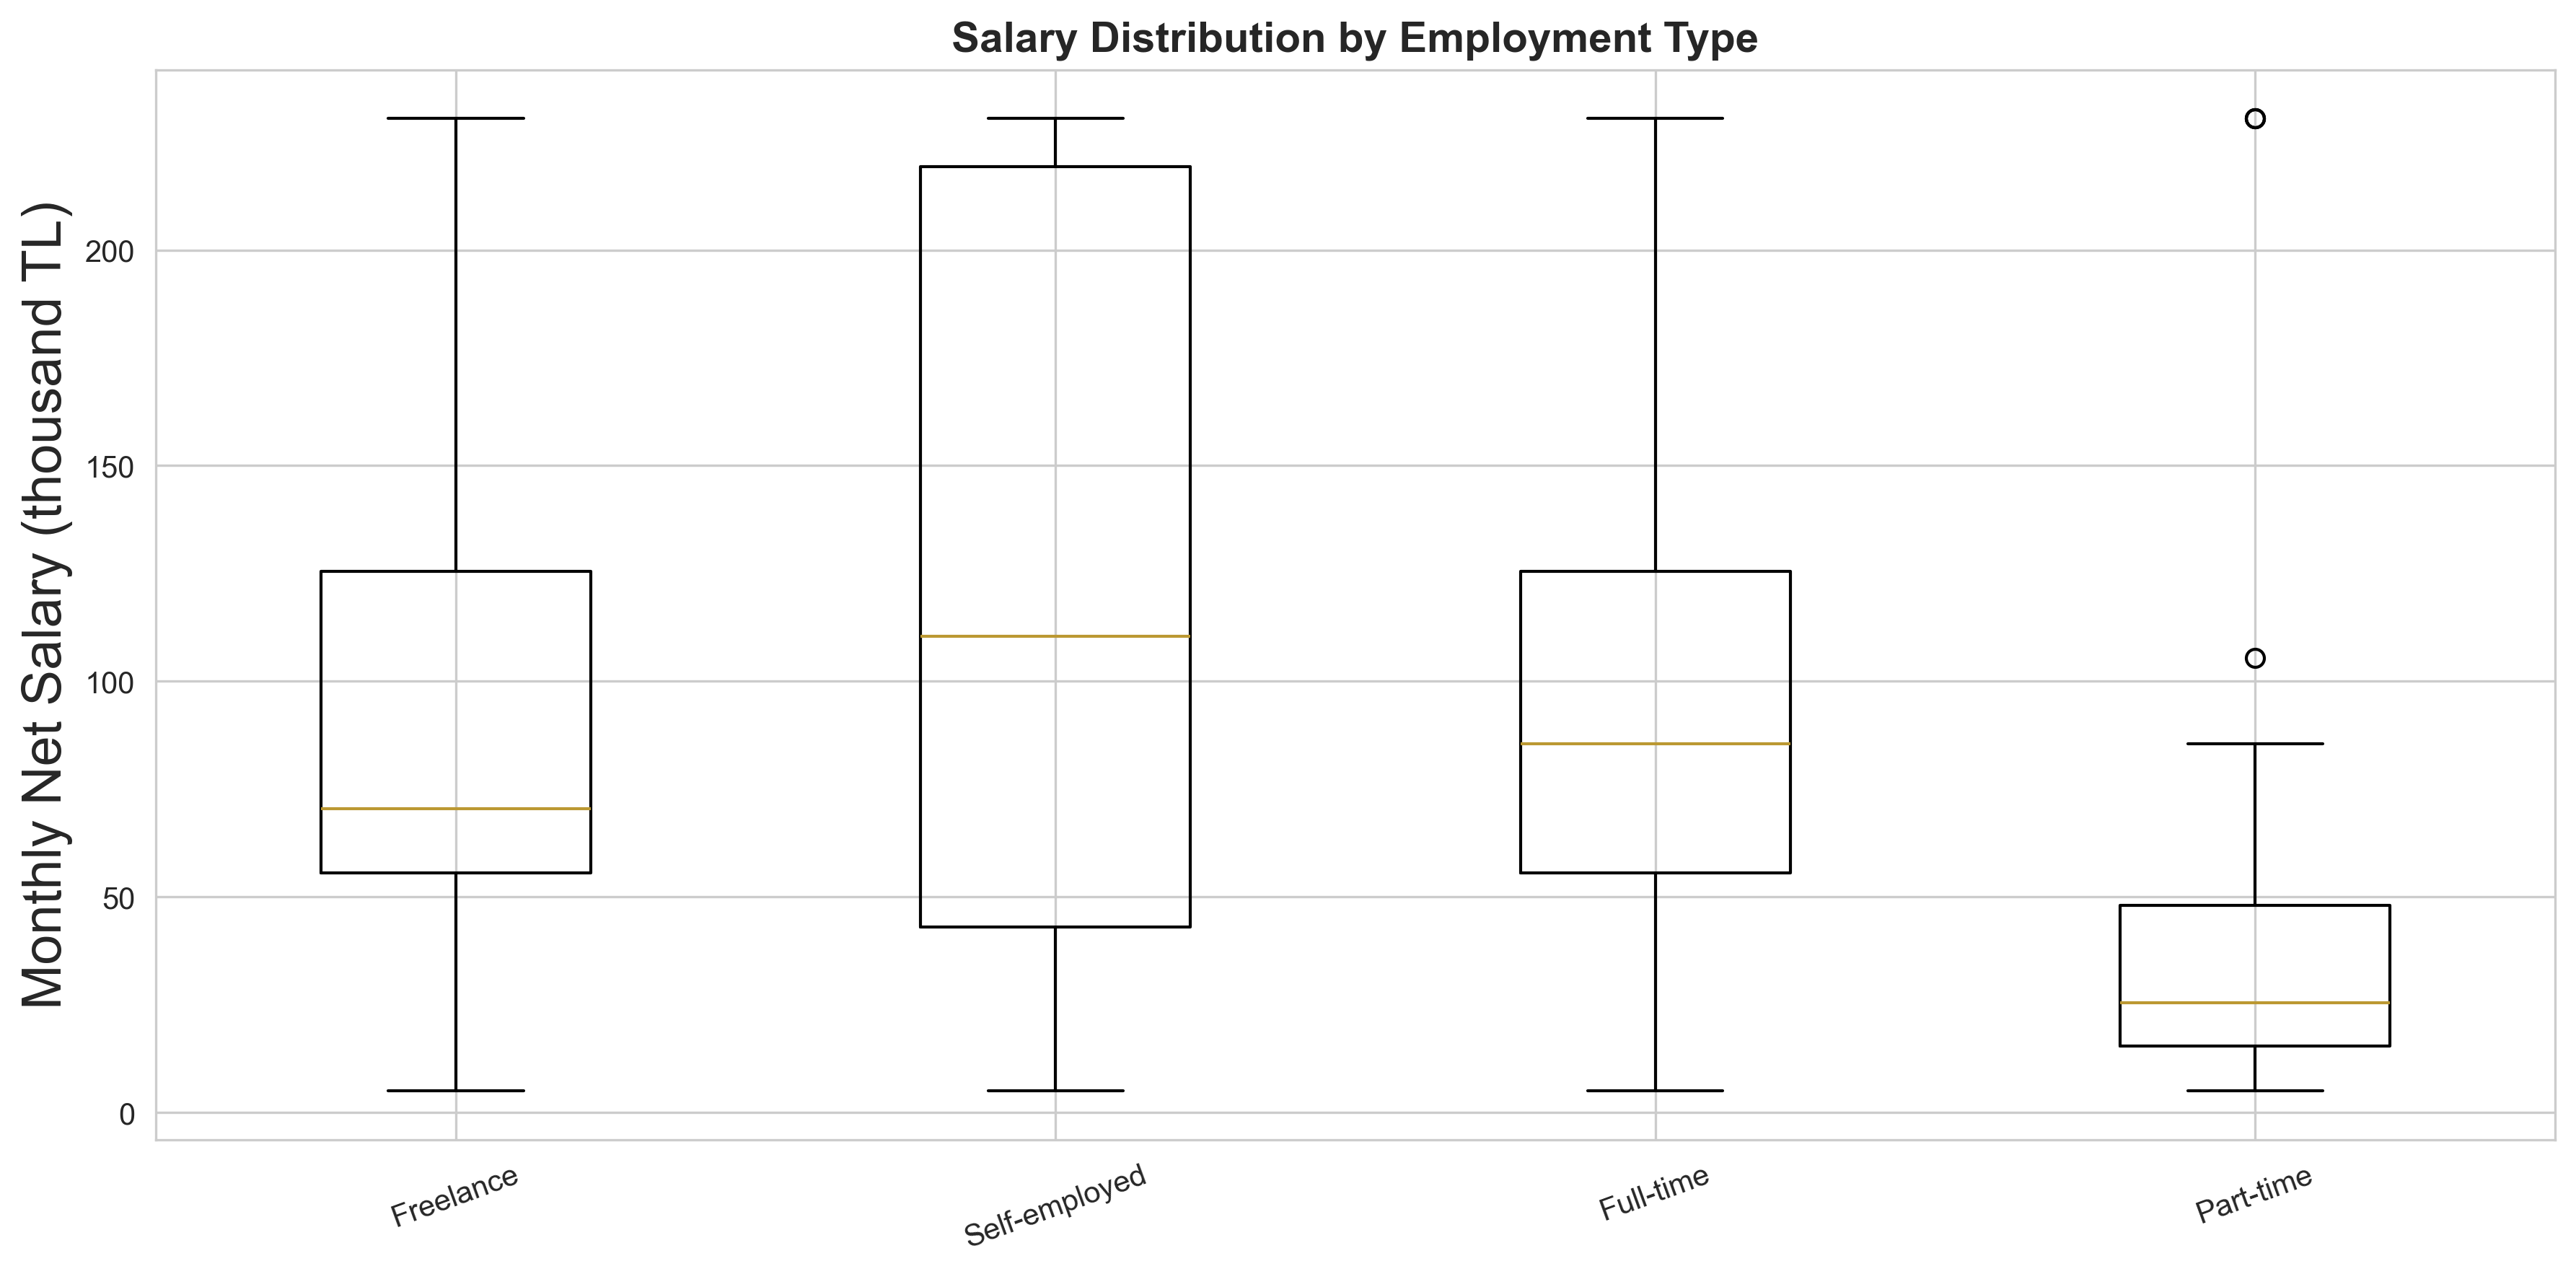
\includegraphics[width=\textwidth]{figures/boxplot_employment_type.png}
    \caption{Salary Distribution by Employment Type - Full-time, part-time, and freelance compensation patterns}
\end{figure}

\textbf{Employment Type Insights:}
\begin{itemize}
    \item \textbf{Full-time Premium:} Traditional employment offers stability and benefits
    \item \textbf{Freelance Flexibility:} Freelance work provides flexibility but variable income
    \item \textbf{Part-time Opportunities:} Part-time roles offer work-life balance trade-offs
    \item \textbf{Self-employment:} Entrepreneurial paths offer highest potential but highest risk
\end{itemize}

\section{React Technology Deep Dive}

\subsection{React vs Non-React Salary Comparison}
Specific analysis of React technology's impact on compensation:

\begin{table}[H]
\centering
\begin{tabular}{lrrr}
\toprule
\textbf{Group} & \textbf{Count} & \textbf{Mean Salary} & \textbf{Difference} \\
\midrule
React Users & 1,008 & 96.1 & \\
Non-React Users & 1,961 & 99.3 & -3.3 \\
\midrule
\textbf{Effect Size} & & & \textbf{Cohen's d = -0.059} \\
\bottomrule
\end{tabular}
\caption{React vs Non-React Salary Comparison}
\end{table}

\textbf{Statistical Significance:} Not significant (p = 0.1289)

\textbf{React Technology Insights:}
\begin{itemize}
    \item \textbf{Market Position:} React remains a valuable skill despite not showing significant premium in this sample
    \item \textbf{Skill Combination:} React combined with other high-ROI technologies may provide better returns
    \item \textbf{Career Strategy:} React knowledge provides foundation for frontend specialization
\end{itemize}

\section{Conclusions and Recommendations}

\subsection{Key Insights Summary}
\begin{enumerate}
    \item \textbf{Remote Work Premium:} Remote workers earn 22.6 thousand TL more (Cohen's d = 0.42), indicating strong market demand for remote talent
    \item \textbf{Geographical Disparity:} European companies offer 70.0 thousand TL higher salaries (Cohen's d = 1.35), representing significant international premium
    \item \textbf{Gender Gap:} Male professionals earn 13.3 thousand TL more (Cohen's d = 0.24), highlighting need for pay equity initiatives
    \item \textbf{Technology Impact:} Specific programming languages provide 15-20\% salary premiums, with Rust offering highest ROI
    \item \textbf{Career Progression:} Clear salary progression from Junior to Senior levels with 40-60\% increases
\end{enumerate}

\subsection{Strategic Recommendations}
\begin{enumerate}
    \item \textbf{For Organizations:}
    \begin{itemize}
        \item Review and address gender pay disparities through transparent compensation policies
        \item Consider remote work policies to attract and retain top talent
        \item Align technology stack decisions with market salary implications
        \item Implement career development programs focused on progression to higher levels
    \end{itemize}
    
    \item \textbf{For Individuals:}
    \begin{itemize}
        \item Focus on high-ROI technologies like Rust for maximum salary impact
        \item Consider remote work opportunities for higher compensation
        \item Target European companies for significant salary increases
        \item Develop specialized skills that combine multiple high-value technologies
    \end{itemize}
    
    \item \textbf{For React Developers:}
    \begin{itemize}
        \item Combine React with high-ROI backend technologies for maximum impact
        \item Focus on full-stack development to increase market value
        \item Consider remote opportunities with international companies
        \item Develop leadership skills for management track progression
    \end{itemize}
\end{enumerate}

\section{Methodological Notes}

\subsection{Data Limitations}
\begin{itemize}
    \item Self-reported salary data may have reporting bias
    \item Sample may not be fully representative of the entire industry
    \item Location data is estimated based on company information
    \item Technology usage is self-reported and may not reflect actual proficiency
    \item Cross-sectional design limits causal inference
\end{itemize}

\subsection{Statistical Methods}
\begin{itemize}
    \item Independent samples t-tests for group comparisons
    \item Cohen's d effect size calculations for practical significance
    \item Multiple comparison corrections where applicable
    \item Correlation analysis for technology-salary relationships
    \item Outlier treatment using IQR and Z-score methods
\end{itemize}

\subsection{Effect Size Interpretation}
\begin{itemize}
    \item \textbf{Small Effect:} Cohen's d = 0.2 (5\% of variance explained)
    \item \textbf{Medium Effect:} Cohen's d = 0.5 (13\% of variance explained)
    \item \textbf{Large Effect:} Cohen's d = 0.8 (26\% of variance explained)
    \item \textbf{Very Large Effect:} Cohen's d = 1.35 (45\% of variance explained)
\end{itemize}

\vspace{2cm}

\begin{center}
\textbf{Report prepared by:} Hakkı Günal\\
\textbf{Data collection period:} August 20-21, 2025\\
\textbf{Total participants:} 2,969 software professionals\\
\textbf{Report generation date:} August 28, 2025\\
\textbf{Key finding:} Remote work provides 22.6 thousand TL premium, European companies offer 70.0 thousand TL more\\
\textbf{Technology insight:} Rust provides highest salary ROI at 69.4 thousand TL
\end{center}

\end{document}
